\chapter{Graph Neural Network Flavour Tagger}\label{chap:gnn_tagger}

Flavour tagging, the identification of jets originating from \bcquarks, is a critical component of the physics programme of the ATLAS experiment at the Large Hadron Collider. 
Current flavour tagging algorithms rely on the outputs of several low-level algorithms, which reconstruct various properties of jets using charged particle tracks, that are then combined using machine learning techniques.
In this note a new machine learning algorithm based on graph neural networks, \GNN, is introduced.
\GNN uses information from a variable number of charged particle tracks within a jet, to predict the jet flavour without the need for intermediate low-level algorithms.
Alongside the jet flavour prediction, the model predicts which physics processes produced the different tracks in the jet, and groups tracks in the jet into vertices.
These auxiliary training objectives provide useful additional information on the contents of the jet and improve performance.
\GNN compares favourably with the current ATLAS flavour tagging algorithms.
For a \bjet efficiency of \pct{70}, the light ($c$)-jet rejection is improved by a factor of \ttbllo (\ttbclo) for jets coming from \ttbar decays with transverse momentum \ttbarpt.
For jets coming from \Zprime decays with transverse momentum \Zprimept, the light ($c$)-jet rejection improves by a factor \zpbllo (\zpbclo) for a comparative \pct{30} \bjet efficiency.



\section{Motivation}\label{sec:gnn_motvation}


\newcommand{\fakesfootnote}{%
A fake track is defined as a track with a truth-matching probability less than $0.5$, where the truth-matching probability is defined in Ref.~\cite{PERF-2015-08}.
}

Flavour tagging, the identification of jets originating from \bcquarks, is a critical component of the physics programme of the ATLAS experiment~\cite{PERF-2007-01} at the Large Hadron Collider (LHC)~\cite{Evans:2008zzb}.
It is of particular importance for the study of the Standard Model (SM) Higgs boson and the top quark, which preferentially decay to \bquarks \cite{HIGG-2018-04,HIGG-2018-13}, and additionally for several Beyond Standard Model (BSM) resonances that readily decay to heavy flavour quarks \cite{EXOT-2019-03}.
The significant lifetime of \bhadrons, approximately $\SI{1.5}{\ps}$ \cite{PhysRevD.98.030001}, provides the unique signature of a secondary decay vertex which has a high mass and is significantly displaced from the primary vertex. Additional signatures of \bhadrons are the tertiary decay vertex, resulting from $b \rightarrow c$ decay chains, and the reconstructed trajectories of charged particles (henceforth simply referred to as tracks) with large impact parameters\footnote{The distance of closest approach from a track to the primary vertex.} (IPs).
These signatures are primarily identified using tracks associated to jets. As such, efficient and accurate track reconstruction is essential for high performance flavour tagging.

This note introduces a novel algorithm, \GNN, which uses Graph Neural Networks (GNNs)~\cite{battaglia2018relational} with auxiliary training objectives, to aid the primary goal of classifying whether jets originate from \ensuremath{b\text{- or }c\text{-quarks}}\xspace(referred to as a flavour tagger). %to identify \ensuremath{b\text{- or }c\text{-jets}}\xspace, . 
The concept is illustrated in \cref{fig:oldvsnew}.
The use of GNNs offers a natural way to classify jets with variable numbers of unordered associated tracks, while allowing for the inclusion of auxiliary training objectives \cite{2020-gnn-for-sv,serviansky2020set2graph}.

\begin{figure}[!htbp]
    \centering
    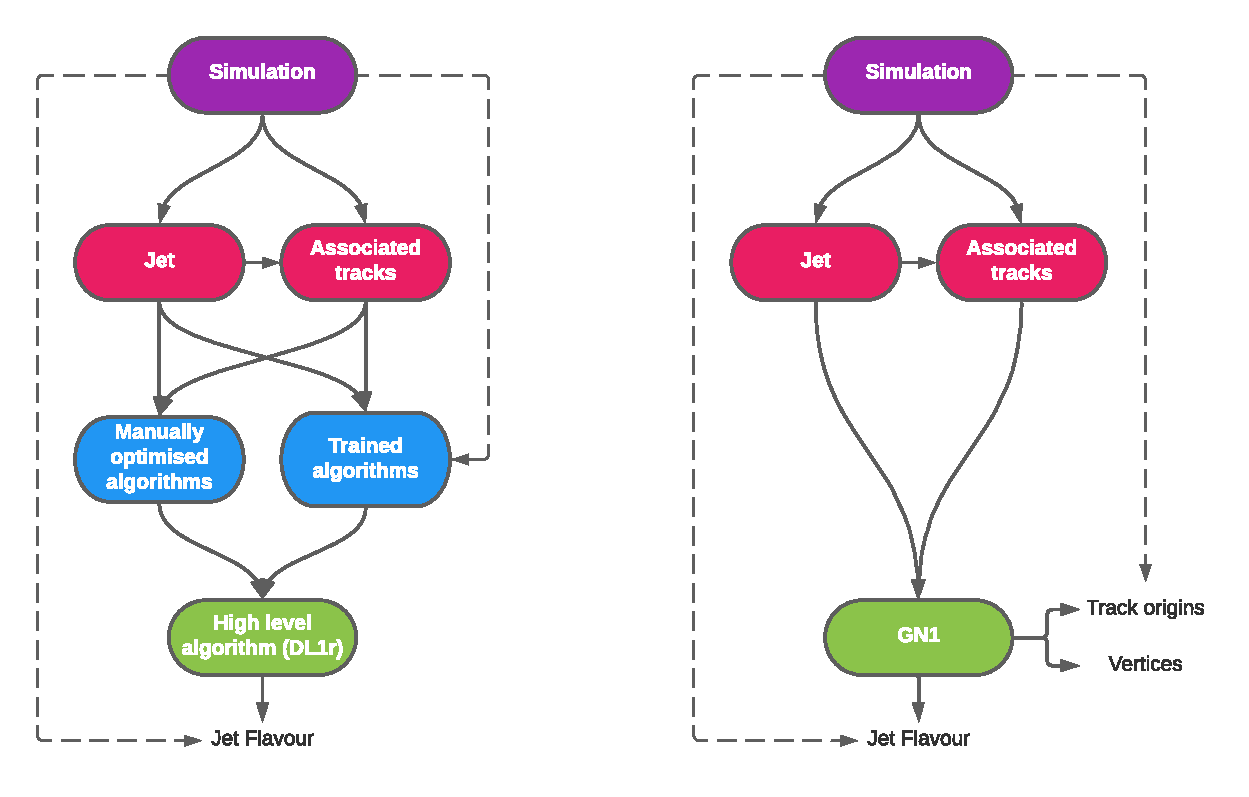
\includegraphics[width=0.8\linewidth]{chapters/gnn_tagger/figs/GNN_compare_contrast.pdf}
    \caption{Comparison of the existing flavour tagging scheme (left) and \GNN (right). The existing approach utilises low-level algorithms (shown in blue), the outputs of which are fed into a high-level algorithm (\DLr). Instead of being used to guide the design of the manually optimised algorithms, additional truth information from the simulation is now being used as auxiliary training targets for \GNN. The solid lines represent reconstructed information, whereas the dashed lines represent truth information.}
    \label{fig:oldvsnew}
\end{figure}

The current ATLAS flavour tagger, \DLr \cite{ATL-PHYS-PUB-2017-013}, is a deep neural network which takes the outputs of a number of independently optimised ``low-level'' algorithms \cite{FTAG-2018-01} as inputs. 
Each of these low-level algorithms makes use of tracks to reconstruct a particular aspect of the experimental signature of heavy flavour jets.
%, for example the presence of secondary vertices (those caused by displaced decays of heavy flavour hadrons).
The low-level algorithms can be manually optimised reconstruction algorithms, for example the SV1 and JetFitter algorithms that reconstruct displaced decay vertices, or trained taggers such as RNNIP and DIPS that use the IPs of a variable number of tracks to identify the flavour of the jet \cite{FTAG-2018-01,ATL-PHYS-PUB-2017-011,ATL-PHYS-PUB-2017-003,ATL-PHYS-PUB-2020-014}.
In contrast \GNN utilises a single neural network, which directly takes the tracks and some information about the jet as inputs. As such, it does not depend on any other flavour tagging algorithm, and a single training of the \GNN fully optimises all aspects of the algorithm.  

\GNN is trained to understand the internal structure of the jet through the use of two auxiliary training objectives: the grouping of tracks originating from a common vertex, and the prediction of the underlying physics process from which each track originated.
These auxiliary objectives are meant to guide the neural network towards a more complete understanding of the underlying physics, removing the need for the low-level algorithms, and therefore simplifying the process of optimising the tagger for new regions of phase space (e.g. \ctag or high-\pt \btag), or when the detector or charged particle reconstruction algorithms are updated.
The training targets for the primary and auxiliary objectives are extracted from “truth information”, i.e. information only available in simulation, as opposed to reconstructed quantities available in both collision data and simulation.

In this note, the following benefits of this approach will be shown:

\begin{enumerate}
    \item Improved performance with respect to the current ATLAS flavour tagging algorithms, with larger background rejection for a given signal efficiency.
    \item The same network architecture can be easily optimised for a wider variety of use cases (e.g. \cjet tagging and high-\pt jet tagging), since there are no low-level algorithms to retune.
    \item There are fewer flavour tagging algorithms to maintain.
    \item Alongside the network's prediction of the jet flavour, the auxiliary vertex and track origin predictions provide more information on why a jet was (mis)tagged or not. This information can also have uses in other applications, for instance to explicitly reconstruct displaced decay vertices or to remove fake tracks.\footnote{\fakesfootnote}
\end{enumerate}

This note is organised as follows: a brief description of the ATLAS detector, object definitions and selections, and samples are provided in \cref{sec:experimental_setup}; details about the model architecture and training procedure are given in \cref{sec:networks}; and results are discussed in \cref{sec:gnn_results}.


\section{Graph Neural Network Theory}\label{sec:gnn_theory}



\section{Experiemental Setup}\label{sec:experimental_setup}

\subsection{Datasets}\label{sec:datasets}

To train and evaluate the model, simulated SM \ttbar and BSM \Zprime events initiated by proton-proton collisions at a center of mass energy $\sqrt{s} = \SI{13}{\TeV}$ are used.
The \Zprime sample is constructed in such a manner that it has a relatively flat jet \pt spectrum up to \SI{5}{\TeV} and decays to an equal numbers of \bcl jets.
The generation of the simulated event samples includes the effect of multiple $pp$ interactions per bunch crossing with an average pileup of $\langle \mu \rangle = 40$, which includes the effect on the detector response due to interactions from bunch crossings before or after the one containing the hard interaction.

\newcommand{\hdampFootnote}{%
The $h_\text{damp}$ parameter is a resummation damping factor and one of the parameters that controls the matching of \textsc{Powheg} matrix elements to the parton shower and thus effectively regulates the high-$p_T$ radiation against which the \ttbar system recoils.}

The \ttbar events are generated using the \textsc{PowhegBox} \cite{powheg2004, powheg2007, powheg2007_2, powheg2010} \textsc{v2} generator at next-to-leading order with the NNPDF3.0NLO \cite{Ball:2014uwa} set of parton distribution functions (PDFs). The $h_\text{damp}$ parameter\footnote{\hdampFootnote} is set to 1.5 times the mass of the top-quark ($m_\text{top}$)~\cite{ATL-PHYS-PUB-2016-020}, with $m_\text{top} = \SI{172.5}{\GeV}$. 
The events are interfaced to \textsc{Pythia}~8.230~\cite{Sjostrand:2014zea} to model the parton shower, hadronisation, and underlying event, with parameters set according to the A14 tune \cite{ATL-PHYS-PUB-2014-021} and using the NNPDF2.3LO set of PDFs \cite{Ball:2012cx}. 
\Zprime events are generated with \textsc{Pythia} 8.2.12 with the same tune and PDF set.
The decays of \bchadrons are performed by \textsc{EvtGen} v1.6.0 \cite{Lange:2001uf}.
Particles are passed through the ATLAS detector simulation \cite{SOFT-2010-01} based on GEANT4 \cite{Agostinelli:2002hh}.

For the \ttbar events, at least one \Wboson boson from the top quark decay is required to decay leptonically.
Truth labelled \bcl jets are kinematically re-sampled in \pt and $\eta$ to ensure identical distributions in these variables. 
The resulting dataset contains \njetstrain jets, \pct{60} of which are \ttbar jets and \pct{40} of which are \Zprime jets.
While \DLr uses \pct{70} \ttbar jets and \pct{30} \Zprime jets, the change in sample composition did not affect the final performance of \GNN.
To evaluate the performance of the model, \njetsval jets from both the \ttbar and \Zprime samples, which are statistically independent from the training sample, are used. 
Track- and jet-level inputs are scaled to have a central value of zero and a variance of unity before training and evaluation. 


\section{Model Architecture}\label{sec:networks}

\subsection{Model Inputs}\label{sec:model-inputs}

\newcommand{\ipdefsfootnote}{%
Impact parameter significances are defined as the IP divided by its corresponding uncertainty, $\dzerosig = d_0 / \dzerouncert$ and $\zzerosig = z_0 / \zzerouncert$.
Track IP significances are lifetime signed according to the track's direction with respect to the jet axis and the primary vertex \cite{PERF-2012-04}.
}

\GNN is given two jet variables and 21 tracking related variables for each track fed into the network.
The jet transverse momentum and signed pseudorapidity constitute the jet-level inputs, with the track-level inputs listed in \cref{tab:track_inputs}.
If a jet has more than 40 associated tracks, the first 40 tracks with the largest transverse IP significance\footnote{\ipdefsfootnote} \dzerosig are selected as inputs.
Full track parameter information and associated uncertainties, along with detailed hit information, carry valuable information about the jet flavour.
In the dense cores of high-\pt jets, tracks are highly collimated and separation between tracks can be of the same order as the active sensor dimensions, resulting in merged clusters and tracks which share hits \cite{PERF-2015-08}.
Due to the relatively long lifetimes of \bhadrons and \chadrons, which can traverse several layers of the ID before decaying and have highly collimated decay products, the presence of shared or missing hits is a critical signature of heavy flavour jets.

Dependence on the absolute value of the azimuthal jet angle $\phi$ is explicitly removed by providing only the azimuthal angle of tracks relative to the jet axis. The track pseudorapidity is also provided relative to the jet axis.

Since heavy flavour hadrons can decay semileptonically, the presence of a reconstructed lepton in the jet carries discriminating information about the jet flavour.
In addition to the baseline \GNN model, the \GNNLep variant includes an additional track-level input, leptonID, which indicates if the track was used in the reconstruction of an electron, a muon or neither. %has a value of $\pm 11$ ($\pm 13$) if the track was used in the reconstruction of an electron (muon), and $0$ otherwise.
The muons are required to be combined \cite{ATL-PHYS-PUB-2015-037}, and the electrons are required to pass the \textit{VeryLoose} likelihood-based identification working point \cite{PERF-2017-01}.

\begin{table}[!htbp]
  \footnotesize\centering
  \setlength{\tabcolsep}{0.5em} % for the horizontal padding
  \caption{
    Input features to the \GNN model.
    Basic jet kinematics, along with information about the reconstructed track parameters and constituent hits are used.
    Shared hits, are hits used on multiple tracks which have not been classified as split by the cluster-splitting neural networks~\cite{PERF-2015-08}, while split hits are hits used on multiple tracks which have been identified as merged.
    A hole is a missing hit, where one is expected, on a layer between two other hits on a track.
    The track leptonID is an additional input to the \GNNLep model.
  }
  \begin{tabular}{ll}
    \toprule 
    \textbf{Jet Input} & \textbf{Description} \\
    \hline
    $\pt$ & Jet transverse momentum \\
    $\eta$ & Signed jet pseudorapidity \\
    \toprule
    \textbf{Track Input} & \textbf{Description} \\
    \hline
    $q/p$ & Track charge divided by momentum (measure of curvature) \\
    $\mathrm{d}\eta$ & Pseudorapidity of the track, relative to the jet $\eta$ \\
    $\mathrm{d}\phi$  & Azimuthal angle of the track, relative to the jet $\phi$ \\
    $d_0$  & Closest distance from the track to the PV in the longitudinal plane \\
    $z_0 \sin\theta$  & Closest distance from the track to the PV in the transverse plane \\
    $\sigma(q/p)$ & Uncertainty on $q/p$ \\
    $\sigma(\theta)$ & Uncertainty on track polar angle $\theta$ \\
    $\sigma(\phi)$  & Uncertainty on track azimuthal angle $\phi$ \\
    $\dzerosig$  & Lifetime signed transverse IP significance \\
    $\zzerosig$  & Lifetime signed longitudinal IP significance \\
    nPixHits   & Number of pixel hits \\
    nSCTHits   & Number of SCT hits \\
    nIBLHits   & Number of IBL hits \\
    nBLHits    & Number of B-layer hits \\
    nIBLShared & Number of shared IBL hits \\
    nIBLSplit  & Number of split IBL hits \\
    nPixShared & Number of shared pixel hits \\
    nPixSplit  & Number of split pixel hits \\
    nSCTShared & Number of shared SCT hits \\
    nPixHoles  & Number of pixel holes \\
    nSCTHoles  & Number of SCT holes \\
    leptonID   & Indicates if track was used to reconstruct an electron or muon \\
    \bottomrule
  \end{tabular}
  \vspace{4mm}
  \label{tab:track_inputs}
\end{table}


Track selection follows the loose selection described in Ref.~\cite{ATL-PHYS-PUB-2020-014} and outlined in~\cref{tab:track_selections}, which was found to improve the flavour tagging performance compared to previous tighter selections, whilst ensuring good resolution of tracks and a low fake rate~\cite{PERF-2015-08}.

\begin{table}[!htbp]
  \footnotesize\centering
  \setlength{\tabcolsep}{0.5em} % for the horizontal padding
  \begin{tabular}{ll}
    \toprule 
    \textbf{Parameter} & \textbf{Selection} \\
    \hline
    $\pt$                & $> 500$ MeV \\
    $|d_0|$              & $< 3.5$ mm \\
    $|z_0 \sin\theta|$   & $< 5$ mm \\
    Silicon hits         & $\ge 8$ \\
    Shared silicon hits  & $< 2$ \\
    Silicon holes        & $< 3$ \\
    Pixel holes          & $< 2$ \\
    \bottomrule
  \end{tabular}
  \caption{
    Quality selections applied to tracks,
    where $d_0$ is the transverse IP of the track, $z_0$ is the longitudinal IP with respect to the PV and $\theta$ is the track polar angle.
    Shared hits are hits used on multiple tracks which have not been classified as split by the cluster-splitting neural networks~\cite{PERF-2015-08}.
    Shared hits on pixel layers are given a weight of 1, while shared hits in the SCT are given a weight of 0.5.
    A hole is a missing hit, where one is expected, on a layer between two other hits on a track.
    }
  \vspace{4mm}
  \label{tab:track_selections}
\end{table}


\subsection{Auxiliary Training Objectives}\label{sec:aux-train-objectives}

In addition to the jet flavour classification, two auxiliary training objectives are defined.
Each auxiliary training objective comes with a training target which, similar to the jet flavour label, are truth labels derived from the simulation.
The presence of the auxiliary training objectives improves the jet classification performance as demonstrated in \cref{sec:gnn_ablations}.

The first auxiliary objective is the prediction of the origin of each track within the jet. 
Each track is labelled with one of the exclusive categories defined in \cref{tab:truth_origins} after analysing the particle interaction that led to its formation. 
Since the presence of different track origins is strongly related to the flavour of the jet, training \GNN to recognise the origin of the tracks may provide an additional handle on the classification of the jet flavour.
This task may also aid the jet flavour prediction by acting as a form of supervised attention~\cite{arxiv.2007.08294}~-~in detecting tracks from heavy flavour decays the model may learn to pay more attention to these tracks.

\begin{table}[!htbp]
  \footnotesize\centering
  \setlength{\tabcolsep}{0.5em} % for the horizontal padding
  \caption{Truth origins which are used to categorise the physics process that led to the production of a track.
            Tracks are matched to charged particles using the truth-matching probability~\cite{PERF-2015-08}.
            A truth-matching probability of less than $0.5$ indicates that reconstructed track parameters are likely to be mismeasured and may not correspond to the trajectory of a single charged particle.
            The ``OtherSecondary'' origin includes tracks from photon conversions, \Kshort and $\Lambda^0$ decays, and hadronic interactions.}
  \begin{tabular}{lll}
      \toprule 
      \textbf{Truth Origin} & \textbf{Description} \\
      \hline
      Pileup  & From a \pp collision other than the primary interaction \\
      Fake    & Created from the hits of multiple particles \\
      Primary & Does not originate from any secondary decay \\
      fromB   & From the decay of a \bhadron \\
      fromBC  & From a \chadron decay, which itself is from the decay of a \bhadron \\
      fromC   & From the decay of a \chadron \\
      %fromTau & From the decay of a $\tau$ \\
      OtherSecondary & From other secondary interactions and decays \\
      \bottomrule
  \end{tabular}
  \vspace{4mm}
  \label{tab:truth_origins}
\end{table}

Displaced decays of \bchadrons lead to secondary and tertiary vertices inside the jet.
Displaced secondary vertices can also occur in \ljets as a result of material interactions and long-lived particle decays (e.g. \Kshort and $\Lambda^0$).
The second auxiliary objective is the prediction of track-pair vertex compatibility. 
For each pair of tracks in the jet, \GNN predicts a binary label, which is given a value 1 if the two tracks in the pair originated from the same point in space, and 0 otherwise. 
To derive the corresponding truth labels for training, truth production vertices within $0.1$ mm are merged.
%, as these are assumed to be unresolvable given the granularity of the ID. 
Track-pairs where one or both of the tracks in the pair have an origin label of either Pileup or Fake are given a label of 0.
Using the pairwise predictions from the model, collections of commonly compatible tracks can be grouped into vertices.
%Two existing low-level tagging algorithms, SV1 and JetFitter, are currently used to find and reconstruct vertices inside jets.
The addition of this auxiliary training objective removes the need for inputs from a dedicated secondary vertexing algorithm.

Both auxiliary training objectives can be considered as ``stepping stones'' on the way to classifying the flavour of the jet. 
By requiring the model to predict the truth origin of each track and the vertex compatibility of each track-pair, the model is guided to learn representations of the jet which are connected to the underlying physics and therefore relevant for classifying the jet flavour. 


%\begin{figure}[!htbp]
%    \centering
%    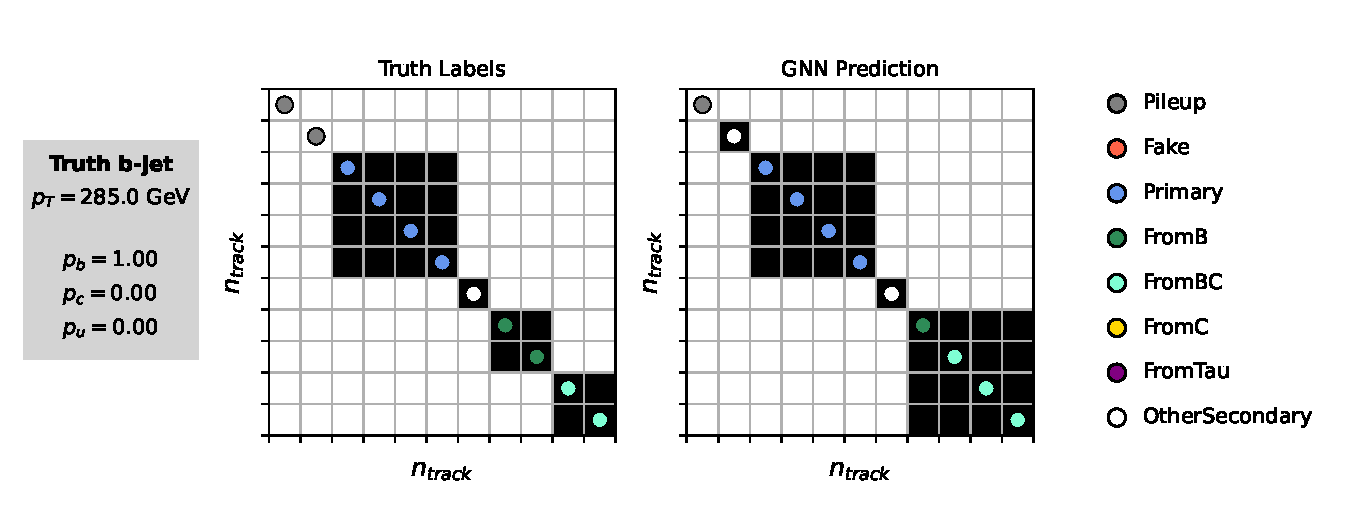
\includegraphics[width=\textwidth]{chapters/gnn_tagger/figs/results/jet_view_1.pdf}
    %\caption{Truth (left) and predicted (right) structure of a \bjet. The shaded black boxes show the grouping of tracks into vertices. In this example, \GNN correctly groups the four primary tracks as having come from a common origin, but does not resolve the $B \rightarrow D$ hadron vertex decay chain. One of the pileup tacks is misidentified as a being OtherSecondary, and one of the $b$ decay tracks is misidentified as being from a $b \rightarrow c$ hadron decay. Nevertheless \GNN correctly predicts the flavour of the jet with a high degree of certainty (class probabilities $p_b$, $p_c$ and $p_u$ are rounded to three significant figures).}
%    \label{fig:jet_view_1}
%\end{figure}
%The auxiliary training objectives also allow for improved model interpretability. 
%\cref{fig:jet_view_1} shows a comparison of the truth origin and vertex information compared with the predicted values from \GNN.
%Such comparisons indicate that \GNN recovers the indended representation of the jet structure, and can also be used to identify limitations.


\subsection{Architecture}\label{sec:Architecture}

As discussed above, the \GNN model combines a graph neural network architecture~\cite{2020-gnn-in-particle-physics} with auxiliary training objectives in order to determine the jet flavour.
Coarse optimisation of the network architecture hyperparameters, for example number of layers and number of neurons per layer, has been carried out to maximise the tagging efficiency.

The model architecture is based on a previous implementation of a graph neural network jet tagger~\cite{serviansky2020set2graph}.
As compared to the previous approach, \GNN uses a only a single graph neural network and makes use of a more sophisticated graph neural network layer \cite{2021arXiv210514491B}, described below.
These changes yield improved tagging performance and a significant reduction in training time with respect to the previous approach.
%the auxiliary classification tasks are performed at the end, along with the graph classification, as opposed to being run half way through the moel and then being fed back in.
%The previous architecture differs from the newer in that it is comprised two graph networks, whereas the newer architecture needs only one.


The model takes jet- and track-level information as inputs, as detailed in \cref{sec:model-inputs}.
The jet inputs are concatenated with each track's inputs, as shown in \cref{fig:model_input_array}.
The combined jet-track vectors are then fed into a per-track initialisation network with three hidden layers, each containing 64 neurons, and an output layer with a size of 64, as shown in \cref{fig:new_arch}. 
The track initialisation network is similar to a Deep Sets model \cite{zaheer2018deep}, but does not include a reduction operation (mean or summation) over the output track representations.
%It allows for initial per-track input processing without the parameter 
%Additionally, other input types with different input sizes can be 

\begin{figure}[!htbp]
    \centering
    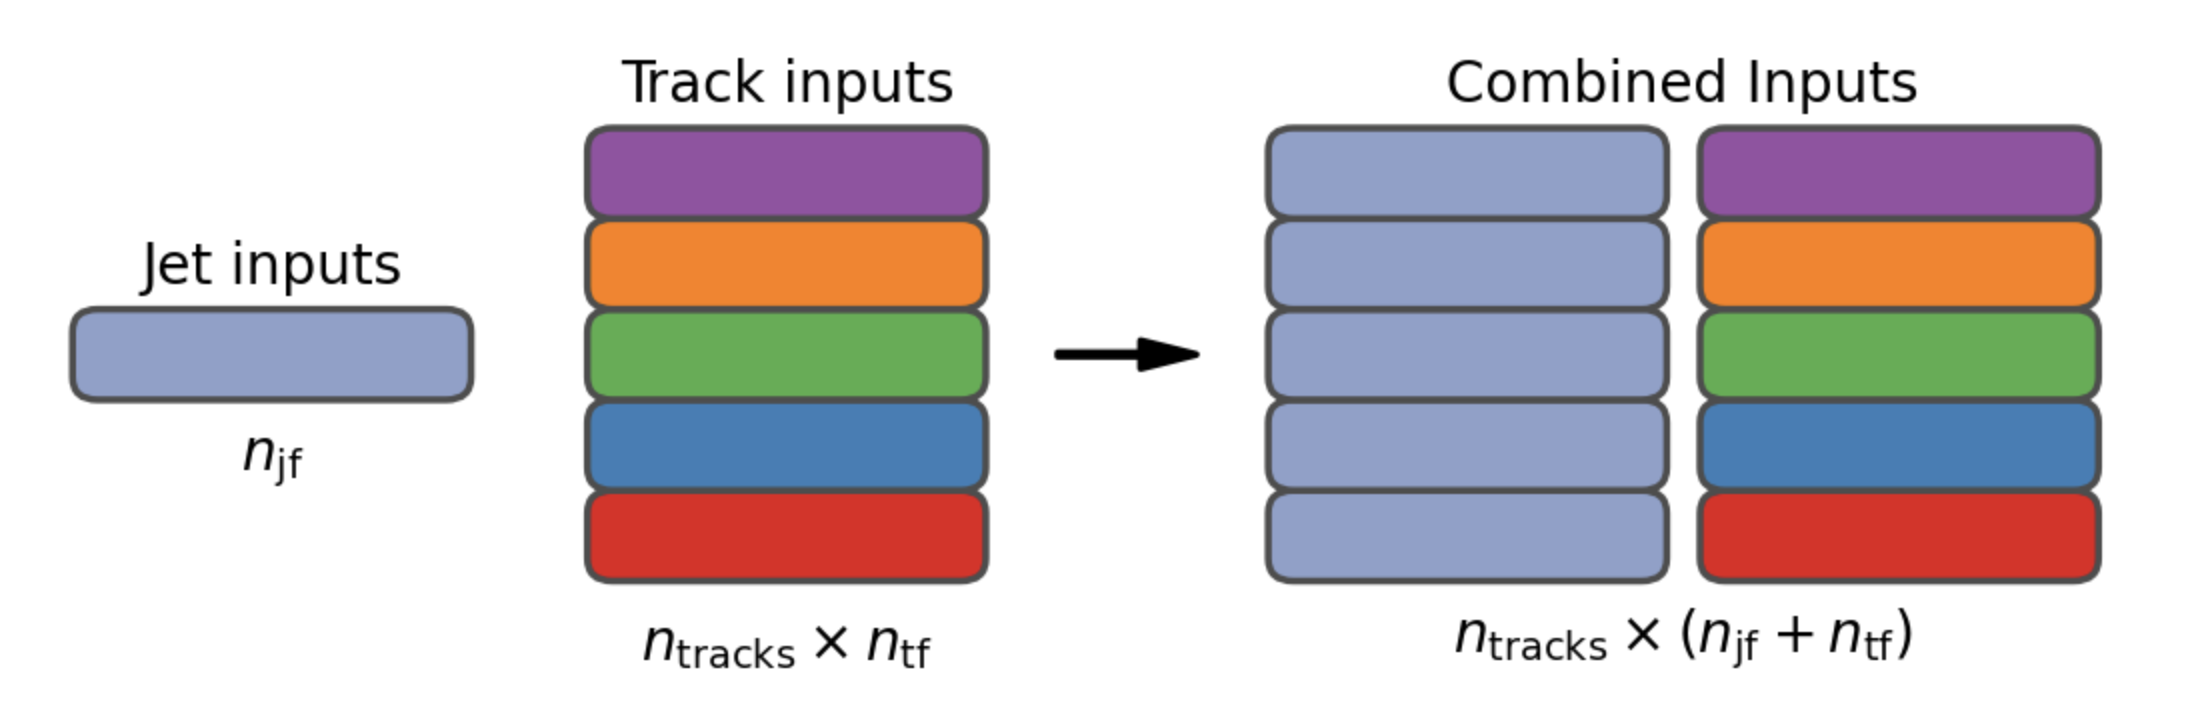
\includegraphics[width=0.6\textwidth]{chapters/gnn_tagger/figs/inputs_diagram.png}
    \caption{The inputs to \GNN are the two jet features ($n_\text{jf} = 2$), and an array of $n_{\text{tracks}}$, where each track is described by 21 track features ($n_\text{tf} = 21$). The jet features are copied for each of the tracks, and the combined jet-track vectors of length 23 form the inputs of \GNN.}
    \label{fig:model_input_array}
\end{figure}

\begin{figure}[!htbp]
    \centering
    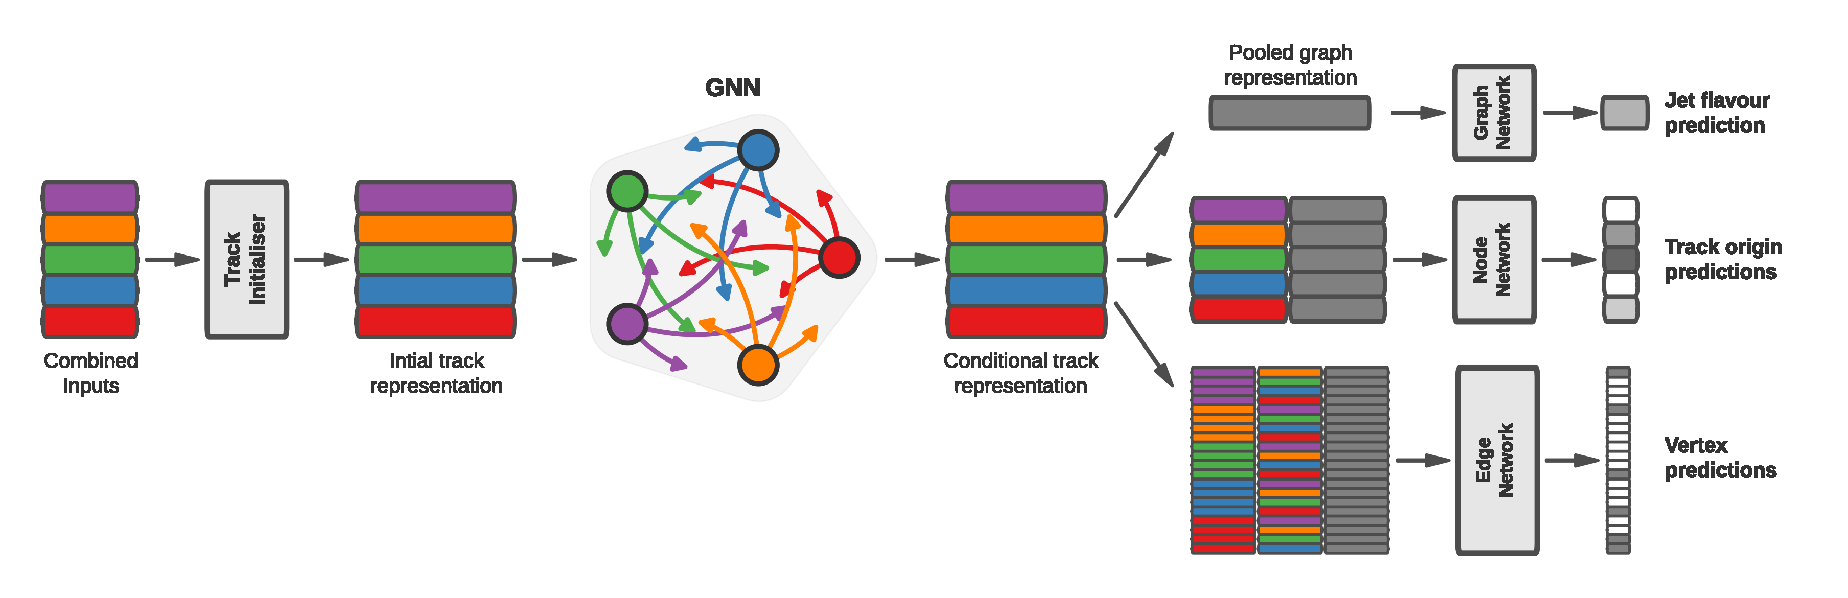
\includegraphics[width=\textwidth]{chapters/gnn_tagger/figs/full_arch.pdf}
    \caption{The network architecture of \GNN. Inputs are fed into a per-track initialisation network, which outputs an initial latent representation of each track. These representations are then used to populate the node features of a fully connected graph network. After the graph network, the resulting node representations are used to predict the jet flavour, the track origins, and the track-pair vertex compatibility.}
    \label{fig:new_arch}
\end{figure}


A fully connected graph is built from the outputs of the track initialisation network, such that each node in the graph neighbours every other node.
Each node $h_i$ in the graph corresponds to a single track in the jet, and is characterised by a feature vector, or representation.
The per-track output representations from the initialisation networks are used to populate the initial feature vectors of each node in the graph.
In each layer of the graph network, output node representations $h_i'$ are computed by aggregating the features of $h_i$ and neighbouring nodes $\mathcal{N}_i$ as described in Ref.~\cite{2021arXiv210514491B}.
First, the feature vectors of each node are fed into a fully connected layer $\mathbf{W}$, to produce an updated representation of each node $\mathbf{W} h_i$.
These updated feature vectors are used to compute edge scores $e(h_i, h_j)$ for each node pair,

\begin{equation}\label{eq:edge_score}
    e(h_i, h_j) = \mathbf{a}^\perp \theta \left[ \mathbf{W}h_i \oplus \mathbf{W}h_j \right],
\end{equation}

where $\oplus$ denotes vector concatenation, $\theta$ is a non-linear activation function, and $\mathbf{a}$ is a learned vector.
These edge scores are then used to calculate attention weights $a_{ij}$ for each pair of nodes using the softmax function over the edge scores

\begin{equation}\label{eq:attention weights}
    a_{ij} = \mathrm{softmax}_j \left[ e(h_i, h_j) \right].
\end{equation}

Finally, the updated node representation $h_i'$ is computed by taking the weighted sum over each updated node representation $\mathbf{W} h_i$, with weights $a_{ij}$

\begin{equation}\label{eq:updated_node_rep}
    h'_i = \sigma \left[ \sum_{j \in \mathcal{N}_i}{a_{ij} \cdot \mathbf{W} {h}_j}  \right].
\end{equation}

The above set of operations constitute a single graph network layer. 
Three such layers are stacked to construct the graph network, representing a balance between achieving optimal performance and preventing overtraining.
The final output node feature vectors from the network are representations of each track that are conditional on the other tracks in the jet.
The output representation for each track is combined using a weighted sum to construct a global representation of the jet, where the attention weights for the sum are learned during training.
Three separate fully connected feedforward neural networks are then used to independently perform the different classification objectives of \GNN.
Each of the objectives makes use of the global representation of the jet.
A summary of the different classification networks used for the various training objectives is shown in \cref{tab:architecture}.

\begin{table}[!htbp]
  \footnotesize\centering
  \setlength{\tabcolsep}{0.5em} % for the horizontal padding
  \caption{
      A summary of GN1's different classification networks used for the different training objectives.
      The hidden layers column contains a list specifying the number of neurons in each layer.
      }
  \begin{tabular}{lll}
      \toprule 
      \textbf{Network} & \textbf{Hidden layers} & \textbf{Output size} \\
      \hline
      Node classification network    & 128, 64, 32 & 7 \\
      Edge classification network    & 128, 64, 32 & 1 \\
      Graph classification network   & 128, 64, 32, 16 & 3 \\
      \bottomrule
  \end{tabular}
  \vspace{4mm}
  \label{tab:architecture}
\end{table}



A node classification network, which takes as inputs the features from a single output node from the graph network and the global jet representation, predicts the track truth origin, as defined in \cref{tab:truth_origins}.
This network has three hidden layers containing 128, 64 and 32 neurons respectively, and an output size of seven, corresponding to the seven different truth origins.

An edge classification network, which takes as inputs the concatenated representations from each pair of tracks and the global jet representation, is used to predict whether the tracks in the track-pair belong to a common vertex.
The edge network has three hidden layers containing 128, 64 and 32 neurons respectively, and a single output, which is used to perform binary classification of the track-pair compatability.
These predictions are used for the auxiliary training objectives discussed in \cref{sec:aux-train-objectives}.

A graph classification network takes only the global jet representation as an input, and predicts the jet flavour. 
The graph classification network is comprised of four fully connected hidden layers with 128, 64, 32 and 16 neurons respectively, and has three outputs corresponding to the \bcl jet classes. 



\subsection{Training}\label{sec:training}

The full \GNN training procedure minimises the total loss function $L_\text{total}$, defined in \cref{eq:loss}. 
This loss is composed of three terms: $L_\text{jet}$, the categorical cross entropy loss over the different jet flavours; $L_\text{vertex}$, the binary track-pair compatability cross entropy loss averaged over all track-pairs; and $L_\text{track}$, the categorical cross entropy loss for the track origin prediction. $L_\text{vertex}$ is computed by averaging over all track-pairs in the batch, and $L_\text{track}$ is computed by averaging over all tracks in the batch.

\begin{equation}\label{eq:loss}
    L_\text{total} = L_\text{jet} + \alpha L_\text{vertex} + \beta L_\text{track}
\end{equation}

The different losses converge to different values during training, reflective of differences in the relative difficulty of the various objectives.
As such, $L_\text{vertex}$ and $L_\text{track}$ are weighted by $\alpha = 1.5$ and $\beta = 0.5$ respectively to ensure they converge to similar values, giving them an equal weighting towards $L_\text{total}$. 
The values of $\alpha$ and $\beta$ also ensure that $L_\text{jet}$ converges to a larger value than $L_\text{vertex}$ and $L_\text{track}$, reflecting the primary importance of the jet classification objective.
In practice, the final performance of the model was not sensitive to modest variations in the loss weights $\alpha$ and $\beta$, or to pre-training using $L_\text{total}$ and fine tuning on the jet classification task only.
As there was a significant variation in the relative frequency of tracks of different origins, the contribution of each origin class to $L_\text{track}$ was weighted by the inverse of the frequency of their occurrence.
In $L_\text{vertex}$, the relative class weight in the loss for track-pairs where both tracks are from either a \borchadron is increased by a factor of two as compared with other track-pairs.

The track classification and vertexing objectives are supplementary to the jet classification objective and trainings can be performed with either the node or edge networks, or both, removed, as discussed in \cref{sec:gnn_ablations}.
In these cases, the corresponding losses $L_\text{vertex}$ and $L_\text{track}$ are removed from the calculation of $L_\text{total}$. 
The resulting trainings demonstrate how useful the different auxiliary training objectives are for the primary jet classification objective.

\GNN trainings are run for \nepochs epochs on 4 NVIDIA V100 GPUs, taking around \minsperepoch mins to complete each epoch over the training sample of \njetstrain jets described in \cref{sec:datasets}.
The Adam optimiser~\cite{arxiv.1412.6980} with an initial learning rate of $1\mathrm{e}{-3}$, and a batch size of 4000 jets (spread across the 4 GPUs) was used.
Typically the validation loss, calculated on \njetsval jets, stabilised after around 60 epochs.
The epoch that minimized the validation loss was used for evaluation.
\GNN has been integrated into the ATLAS software~\cite{ATL-SOFT-PUB-2021-001} using ONNX~\cite{bai2019}, and jet flavour predictions for the test sample are computed using the ATLAS software stack.
%\todo{inlcude loss vs epoch? or save for paper}


\section{Results}\label{sec:gnn_results}


The performance of the \GNN tagger is evaluated for both \btag and \ctag use cases, and for both jets with \ttbarpt from the \ttbar sample and jets with \Zprimept from the \Zprime sample.
Performance is compared to the \DLr tagger \cite{ATL-PHYS-PUB-2017-013}, which has been retrained on 75 million jets from the same samples as \GNN.
%Sample prepration is identical for the different models.
The input RNNIP tagger \cite{ATL-PHYS-PUB-2017-003} to \DLr has not been retrained.
%\DLr is a modification of the previous \DLr tagger \cite{ATL-PHYS-PUB-2017-013} which which replaces RNNIP with DIPS, a separately trained track-based algorithm based on deep sets. 
%The DIPS tagger uses the loose track selection defined in \cite{ATL-PHYS-PUB-2020-014}.

The taggers predict the probability that a jet belongs to the \bcl classes. To use the model for \btag, these probabilities are combined into a single score \Db, defined as

\begin{equation}\label{eq:btag-disc}
    \Db = \log{\frac{p_b}{(1-\fc )p_l + \fc  p_c}} ,
\end{equation}

where \fc is a free parameter that determines the relative weight of $p_c$ to $p_l$ in the score \Db, controlling the trade-off between $c$- and \lrej performance.
This parameter is set to a value of $\fc = 0.018$ for the \DLr model, obtained through an optimisation procedure designed to maximise the \clrej of \DLr \cite{ATL-PHYS-PUB-2017-013}.
For the \GNN models a value of $\fc = 0.05$ is used, based on a similar optimisation procedure.
The choice of \fc is arbitrary, with the different optimised values reflecting the relative $c$- versus light-jet rejection performance of the various taggers.
A fixed-cut working point (WP) defines the corresponding selection applied to the tagging discriminant \Db in order to achieve a given inclusive efficiency on the \ttbar sample.

The technical implementation of \GNN results in any jet with no associated tracks or exactly one associated track to be classified as a \ljet.
The impact of this on the tagging performance of \GNN was found to be negligible, with \pct{0.12} of \ttbarbjets and \pct{0.02} of \Zprimebjets affected.
Of those, \pct{89} of the \ttbarbjets and \pct{98} of the \Zprimebjets are classified as \ljets by \DLr at the \pct{70} \ttbar WP.

A comparison of the \btag discriminant \Db between \DLr and \GNN is given in \cref{fig:ttbar_btag_disc}. 
The shapes of the distributions are broadly similar for \bcl jets, however, the \GNN model shifts the \bjet distribution to higher values of \Db in the regions with the best discrimination.
The \GNN \cjet distribution is also shifted to lower values of \Db when compared with \DLr, enhancing the separation and indicating that \GNN will improve \cjet rejection when compared with \DLr.

\begin{figure}[!htb]
    \centering
    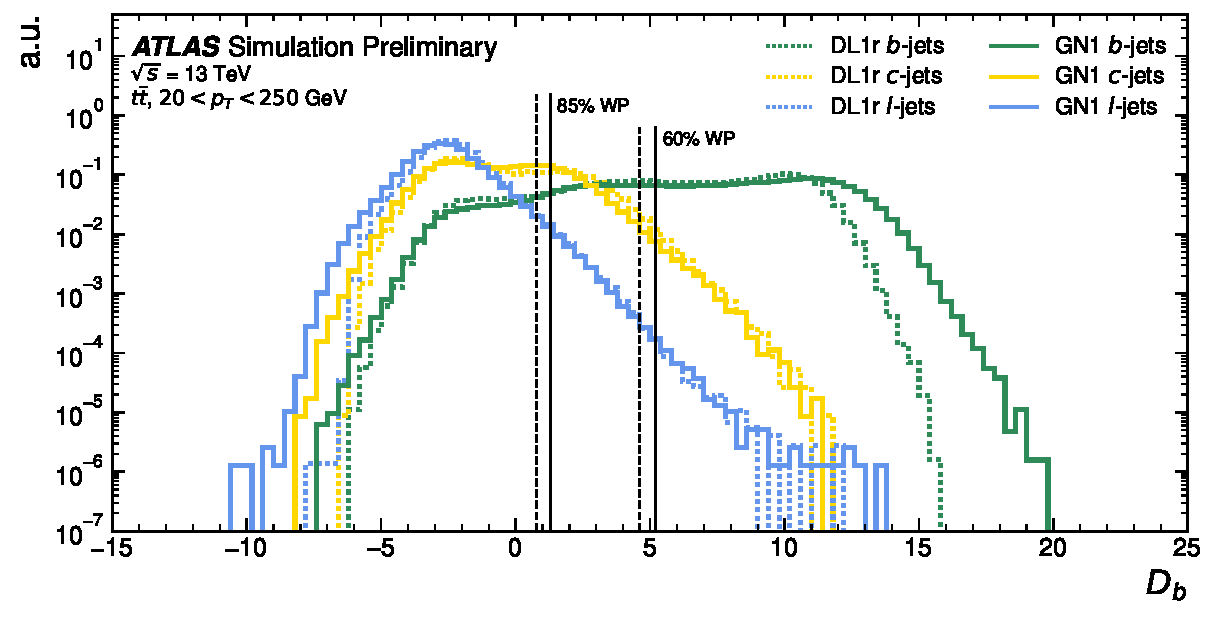
\includegraphics[width=0.6\textwidth]{chapters/gnn_tagger/figs/results/main/ttbar/ttbar_score_DL1r_GN120220509_btag.pdf}
    \caption{Comparison between the \DLr and \GNN \btag discriminant \Db for jets in the \ttbar sample.
    The \pct{85} WP and the \pct{60} WP are marked by the solid (dashed) lines for \GNN (\DLr), representing respectively the loosest and tightest WPs used by analyses.
    A value of $\fc = 0.018$ is used in the calculation of \Db for \DLr and $\fc = 0.05$ is used for \GNN. The distributions of the different jet flavours have been normalised to unity area.}
    \label{fig:ttbar_btag_disc}
\end{figure}



\subsection{\texorpdfstring{\btagging}{b-tagging} Performance}\label{sec:gnn_btag_perf}

The performance of a \btag algorithm is quantified by its power to reject \cljets for a given $b$-jet tagging efficiency, or WP. 
In order to compare the \btag performance of the different taggers for the $b$-jet tagging efficiencies in the range typically used by analyses, the corresponding \clrej rates are displayed in \cref{fig:ttbar_btag_roc,fig:zprime_btag_roc} for jets in the \ttbar and \Zprime samples respectively.
Four standard WPs with $b$-jet tagging efficiencies of \pct{60}, \pct{70}, \pct{77} and \pct{85} are used by physics analyses depending on their specific signal and background requirements.
These WPs are defined using \ttbarjets only.
The $b$-jet tagging efficiencies for \Zprimejets are lower than the corresponding WPs calculated in the \ttbar sample, due to the much higher jet \pt range in the \Zprime sample.
For instance the WP defined to provide a $70\%$ $b$-jet tagging efficiency on the \ttbar sample results in a $b$-jet tagging efficiency of $\sim30\%$ on the \Zprime sample.
To account for this, the range of $b$-jet tagging efficiencies displayed in \cref{fig:zprime_btag_roc} is chosen to span the lower values achieved in the \Zprime sample.

For \ttbarjets with \ttbarpt, \GNN demonstrates considerably better \clrej compared with \DLr across the full range of $b$-jet tagging efficiencies probed.
The relative improvement depends on the \bjet tagging efficiency, with the largest improvements found at lower values.
At a $b$-jet tagging efficiency of \pct{\ttlo}, the \crej improves by a factor of \ttbclo and the \lrej improves by a factor of \ttbllo with respect to \DLr.
For high-\pt \Zprimejets with \Zprimept, \GNN also brings considerable performance improvements with respect to \DLr across the range of $b$-jet tagging efficiencies studied.
Again, the largest relative improvement in performance comes at lower $b$-jet tagging efficiencies.
At a $b$-jet tagging efficiency of \pct{\zplo}, \GNN improves the \crej by a factor of \zpbclo and the \lrej by a factor of \zpbllo.
An increasing statistical uncertainty due to the high rejection of background affects the comparison at lower $b$-jet tagging efficiencies.
It is estimated that for a $b$-jet tagging efficiency of $70\%$ in the \ttbar sample, $\sim5\%$ ($\sim30\%$) of the relative improvement in the $c$-jet (light-jet) rejection comes from loosening the track selection and for a $b$-jet tagging efficiency of $30\%$ in the \Zprime the corresponding number is $\sim10\%$ for both $c$-jets and light-jets.
Given the sophisticated exploitation of low-level information, further studies are needed to confirm if the performance gain is also observed in experimental data.

The \GNNLep variant shows improved performance with respect to the baseline \GNN model, demonstrating the additional jet flavour discrimination power provided by the leptonID track input.
For \ttbarjets, the relative \crej improvement with respect to \DLr at the \bWP{\ttlo} increases from a factor of \ttbclo for \GNN to a factor of $\sim 2.8$ for \GNNLep.
The improvement in \lrej also increases from a factor of \ttbllo to $\sim 2.5$ at this WP.
For \Zprimejets, the relative \crej (\lrej) improvement with respect to \DLr increases from a factor of \zpbclo to $\sim 3$ (\zpbllo to $\sim 7.5$) at a $b$-jet tagging efficiency of \pct{\zplo}.
As shown in \cref{fig:vs_pt_flat_leff}, the greatest improvement of \GNNLep over \GNN is seen at low \pt.

\begin{figure}[!p]
    \centering
    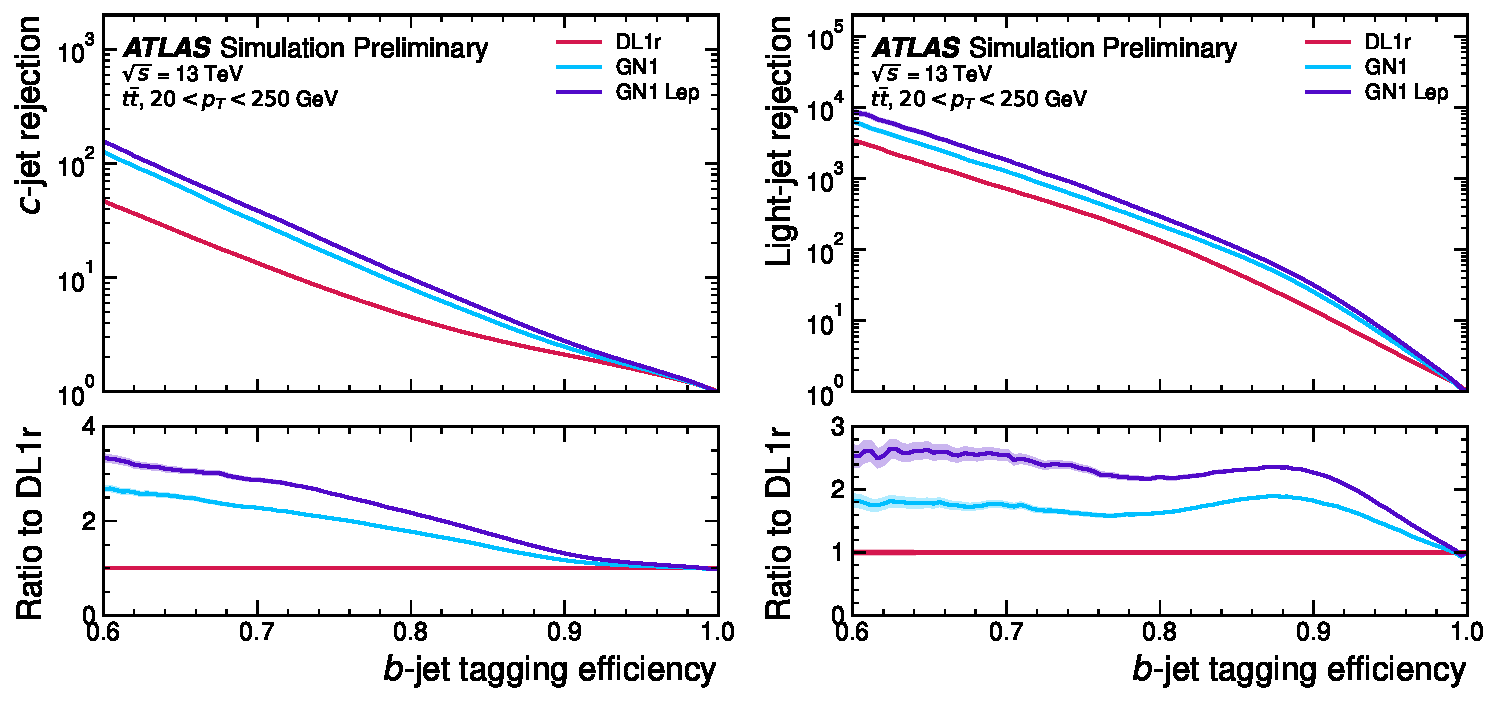
\includegraphics[width=\textwidth]{chapters/gnn_tagger/figs/results/main/ttbar/ttbar_roc_btag.pdf}
    \caption{The \cjet (left) and \ljet (right) rejections as a function of the $b$-jet tagging efficiency for \ttbarjets with \ttbarpt.
             The ratio with respect to the performance of the \DLr algorithm is shown in the bottom panels.
             A value of $\fc = 0.018$ is used in the calculation of \Db for \DLr and $\fc = 0.05$ is used for \GNN and \GNNLep.
             Binomial error bands are denoted by the shaded regions.
             At \bjet tagging efficiencies less than $\sim$\pct{75}, the \lrej becomes so large that the effect of the low number of jets is visible.
             The lower $x$-axis range is chosen to display the \bjet tagging efficiencies usually probed in these regions of phase space.}
    \label{fig:ttbar_btag_roc}
\end{figure}

\begin{figure}[!p]
    \centering
    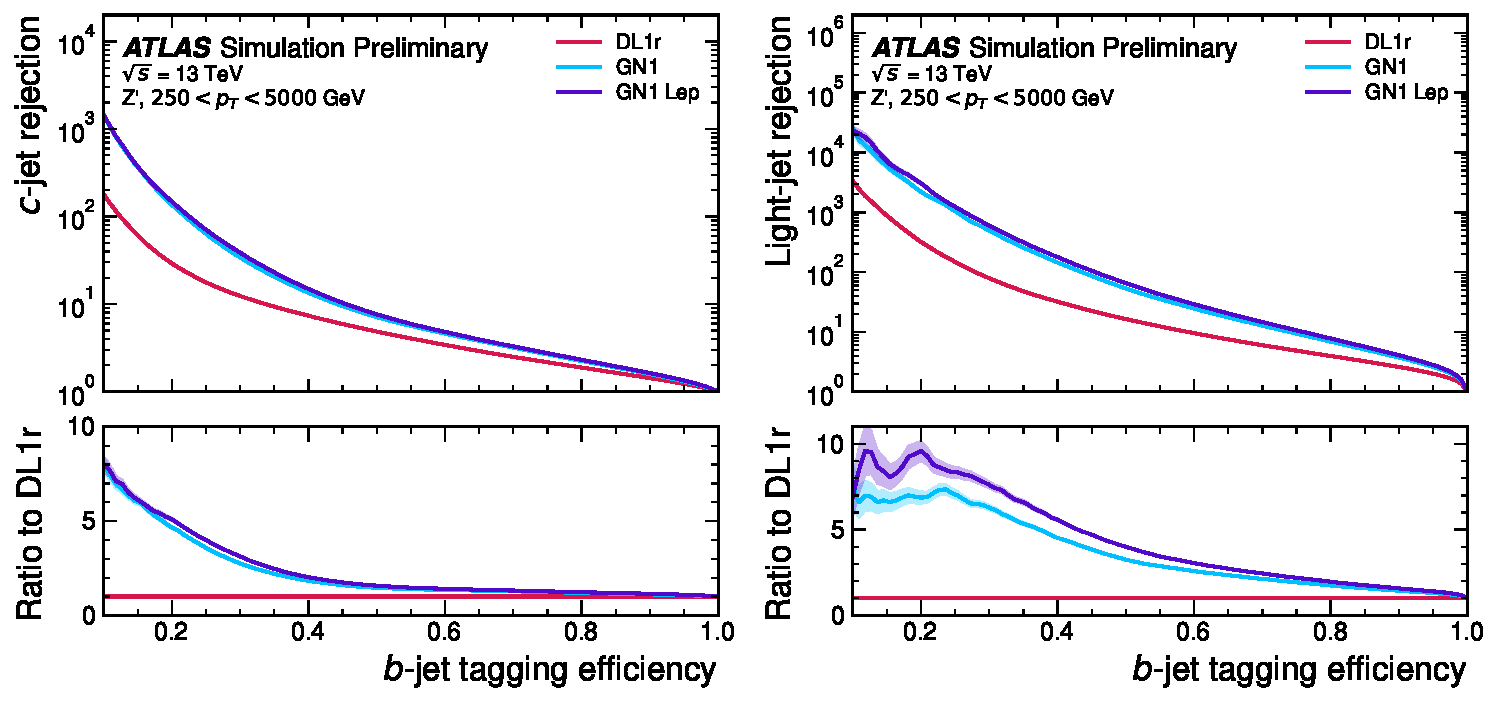
\includegraphics[width=\textwidth]{chapters/gnn_tagger/figs/results/main/zprime/zprime_roc_btag.pdf}
    \caption{The \cjet (left) and \ljet (right) rejections as a function of the $b$-jet tagging efficiency for \Zprimejets with \Zprimept.
             The ratio with respect to the performance of the \DLr algorithm is shown in the bottom panels.
             A value of $\fc = 0.018$ is used in the calculation of \Db for \DLr and $\fc = 0.05$ is used for \GNN and \GNNLep.
             Binomial error bands are denoted by the shaded regions.
             At \bjet tagging efficiencies less than $\sim$\pct{20}, the \lrej becomes so large that the effect of the low number of jets is visible.
             The lower $x$-axis range is chosen to display the \bjet tagging efficiencies usually probed in these regions of phase space.}
    \label{fig:zprime_btag_roc}
\end{figure}

The performance of the taggers is strongly dependent on the jet \pt.
Charged particle reconstruction is particularly challenging within high-\pt jets \cite{PERF-2015-08}.
The multiplicity of fragmentation particles increases as a function of \pt, while the number of particles from heavy flavour decays stays constant.
Collimation of particles inside the jet increases and approaches the granularity of the tracking detectors, making it difficult to resolve the trajectories of different particles.
Furthermore, at high \pt, heavy flavour hadrons will travel further into the detector before decaying.
For hadrons which traverse one or more layers of the ID before decaying, the corresponding decay tracks may pick up incorrect hits, left by the hadron itself or fragmentation particles, in the inner layers of the detector, reducing the accuracy of the reconstructed track parameters.
These factors contribute to a reduced reconstruction efficiency for heavy flavour tracks, and a general degradation in quality of tracks inside the core of a jet, which in turn reduces the jet classification performance.

% In order to study how the \bseleff of the taggers varies as a function of jet \pt, the \beff for \ttbarZprimejets at a fixed \pct{77} \ttbar WP is shown in as a function of \pt in \cref{fig:vs_pt_fixed_ttbar}.
% For \ttbarjets, the different taggers perform similarly in the different \pt bins.
% Performance for jets with $\pt < \SI{100}{\GeV}$ is lower than jets with $\pt > \SI{100}{\GeV}$ due to the shorter flight distance of the \bhadron in low \pt jets.
% For \Zprimejets at the \pct{77} \ttbar WP, the efficiency for each of the taggers starts high at around \pctr{60}{70} for $\pt < \SI{1}{\TeV}$, and then drops with increasing \pt, beginning to plateau at around \pctr{5}{15} above \SI{4}{\TeV}.
% At low $\pt < \SI{500}{\GeV}$, the \beff at a fixed \leff for \DLr (\GNN) is \pct{65} (\pct{75}), and this drops to approximately \pct{10} (\pct{20}) as the jet \pt moves to extreme ranges of up to $\pt > \SI{4}{\TeV}$.
% At \SI{1}{\TeV}, \GNN improves the \beff at a fixed \ceff (\leff) as compared with \DLr by \pct{10} (\pct{20}).
% Above \SI{4}{\TeV}, the relative increase in \bjet tagging efficiency between \DLr and \GNN is larger, with increases of up to \pct{30} (\pct{80}) at a fixed \crej (\lrej).

% The \bseleff of the \GNNLep variant is similar to the baseline \GNN model for both \ttbarZprimejets at the \pct{77} \ttbar WP.
In order to study how the $b$-jet tagging efficiency of the taggers varies as a function of jet \pt, the $b$-jet tagging efficiency as a function of \pt for a fixed light-jet rejection of 100 in each bin is shown in \cref{fig:vs_pt_flat_leff}.
For \ttbarjets, at a fixed \ljet rejection of 100, \GNN improves the $b$-jet tagging efficiency by approximately \pct{4} across all jet \pt bins.
\GNNLep shows improved performance with respect to \GNN, in particular at lower \pt, with the relative increase in the $b$-jet tagging efficiency going from \pct{4} to \pct{8}.
For \Zprimejets, \GNN has a higher $b$-jet tagging efficiency than \DLr across the \pt range, with the largest relative improvement in performance, approximately a factor of 2, found at jet $\pt > \SI{2}{\TeV}$.
\GNN outperforms \DLr across the entire jet \pt spectrum studied. 
The performance was also evaluated as a function of the average number of pileup interactions in an event, and was found to have no significant dependence on this quantity.

% \begin{figure}[!p]
%     \centering
%     \begin{subfigure}[b]{0.48\textwidth}
%         \centering
%         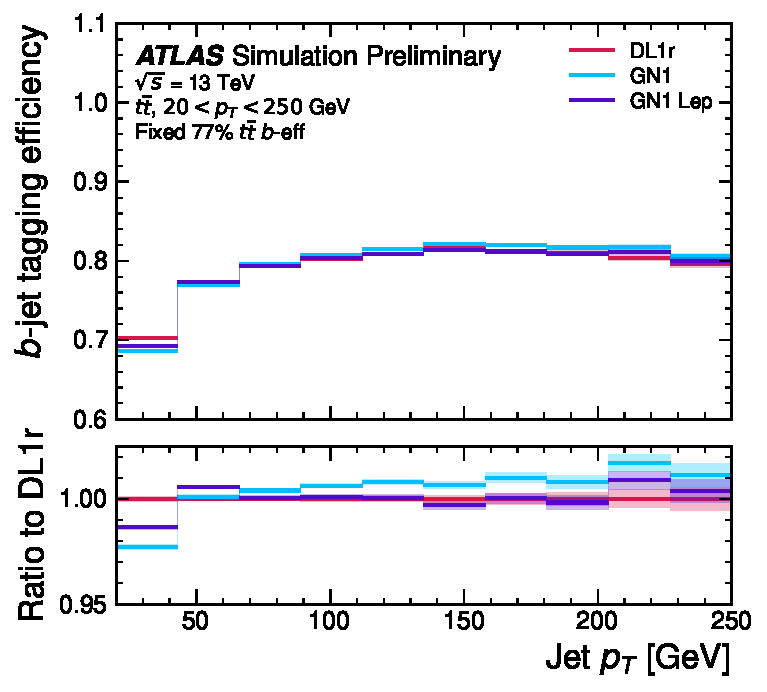
\includegraphics[width=\textwidth]{chapters/gnn_tagger/figs/results/main/ttbar/ttbar_fixed_beff_by_pt_btag.pdf}
%         %\caption{sub}
%         %\label{fig:sub}
%     \end{subfigure}
%     \quad
%     \begin{subfigure}[b]{0.48\textwidth}
%         \centering
%         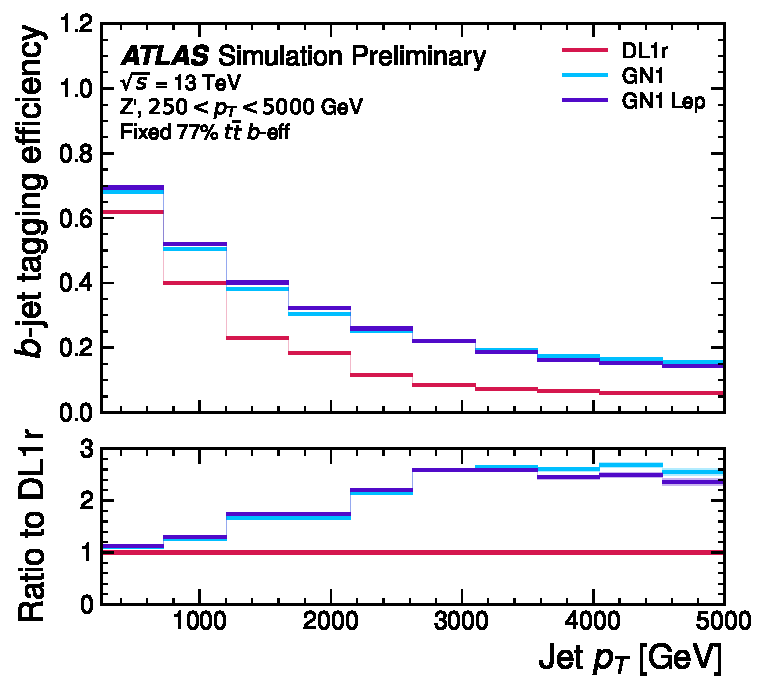
\includegraphics[width=\textwidth]{chapters/gnn_tagger/figs/results/main/zprime/zprime_fixed_beff_by_pt_btag.pdf}
%         %\caption{sub}
%         %\label{fig:sub}
%     \end{subfigure}
%     \caption{The \btag efficiency for \ttbarjets (left) and \Zprime jets (right) as a function of jet \pt for a fixed \pct{77} \ttbar \beff.
%              For \ttbarjets, the taggers show a similar response in the different \pt bins.
%              For \Zprimejets, performance drops off with increasing \pt for all taggers, though \GNN improves the \beff by up to a factor of 2.5 for jets with $\pt > \SI{3}{\TeV}$.
%              The standard error on the mean is shown in the shaded regions.
%              }
%     \label{fig:vs_pt_fixed_ttbar}
% \end{figure}


\begin{figure}[!htbp]
    \centering
    \begin{subfigure}[b]{0.48\textwidth}
        \centering
        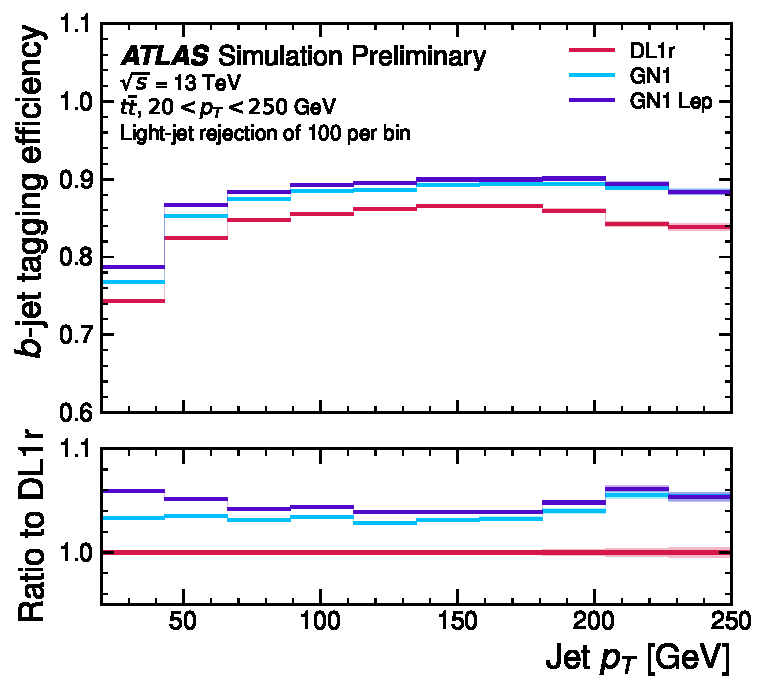
\includegraphics[width=\textwidth]{chapters/gnn_tagger/figs/results/main/ttbar/ttbar_flat_leff_by_pt_btag.pdf}
        %\caption{sub}
        %\label{fig:sub}
    \end{subfigure}
    \quad
    \begin{subfigure}[b]{0.48\textwidth}
        \centering
        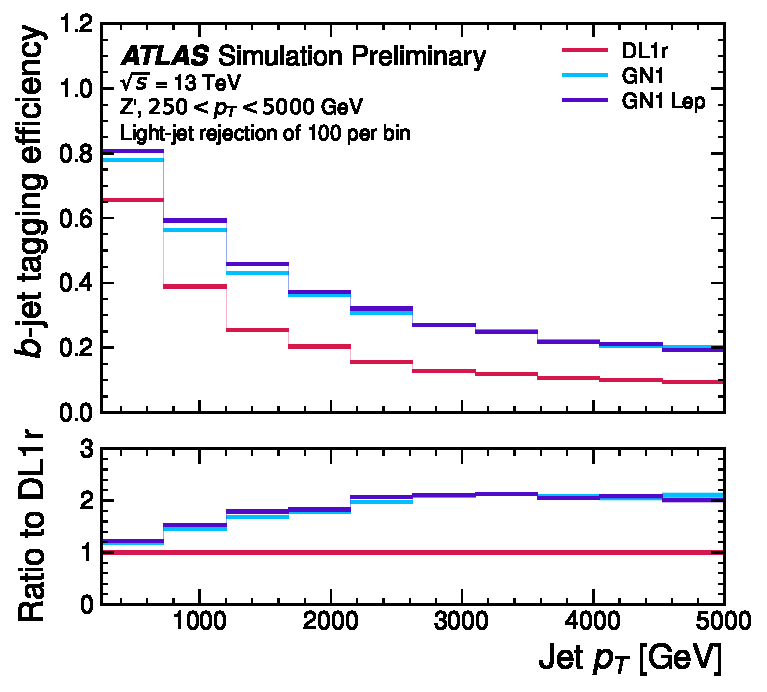
\includegraphics[width=\textwidth]{chapters/gnn_tagger/figs/results/main/zprime/zprime_flat_leff_by_pt_btag.pdf}
        %\caption{sub}
        %\label{fig:sub}
    \end{subfigure}
    \caption{The \bjet tagging efficiency for \ttbarjets (left) and \Zprimejets (right) as a function of jet \pt with a fixed \ljet rejection of 100 in each bin.
             %For \ttbarjets, \GNN increases \beff by approximately \pct{5} with respect to \DLr in each \pt bin.
             %For \Zprimejets, \GNN increases \beff by up to a factor of 2 for jets with $\pt > \SI{2.5}{\TeV}$ with respect to \DLr.
             A value of $\fc = 0.018$ is used in the calculation of \Db for \DLr and $\fc = 0.05$ is used for \GNN and \GNNLep.
             %\GNN demonstrates improved performance with respect to \DLr accross the \pt range.
             Binomial error bands are denoted by the shaded regions.
             }
    \label{fig:vs_pt_flat_leff}
\end{figure}




\subsection{\texorpdfstring{\ctagging}{c-tagging} Performance}\label{sec:gnn_ctag_perf}

Since \GNN does not rely on any manually optimised low-level tagging algorithms, which may not have been optimised for \ctag, tagging \cjets presents a compelling use case for \GNN.
To use the model for \ctag, the output probabilities are combined into a single score \Dc, defined similarly to \cref{eq:btag-disc} as

\begin{equation}\label{eq:ctag-disc}
    D_c = \log{\frac{p_c}{(1-f_b)p_l + f_b p_b}} .
\end{equation}

A value of $\fb = 0.2$ is used for all models.
Similar to \cref{sec:gnn_btag_perf}, performance of the different taggers is compared by scanning through a range of $c$-jet tagging efficiencies and plotting the corresponding \blrej rates.
As in \cref{sec:gnn_btag_perf}, WPs are defined using \ttbarjets.
Standard $c$-jet tagging efficiency WPs are significantly lower in comparison with the \btag WPs in order to maintain reasonable $b$- and light-jet rejection rates.
This is reflected in the range of $c$-jet tagging efficiencies used in \cref{fig:ttbar_ctag_roc,fig:zprime_ctag_roc}.
In \cref{fig:ttbar_ctag_roc}, which displays the \ctag performance of the models on the \ttbarjets, \GNN performs significantly better than \DLr.
The \blrej improve most at lower $c$-jet tagging efficiencies, with both background rejections increasing by a factor of 2 with respect to \DLr at a $c$-jet tagging efficiency of \pct{25}.
\GNNLep outperforms \GNN, with the \brej (\lrej) relative improvement increasing from a factor of 2 to 2.1 (2 to 2.3) at the \WP{25}{c}.
\cref{fig:zprime_ctag_roc} shows the \ctag performance on the \Zprimejets.
Both \GNN and \GNNLep perform similarly, improving the \brej by \pct{60} and the \lrej by a factor of 2 at the \WP{25}{c}.

\begin{figure}[!p]
    \centering
    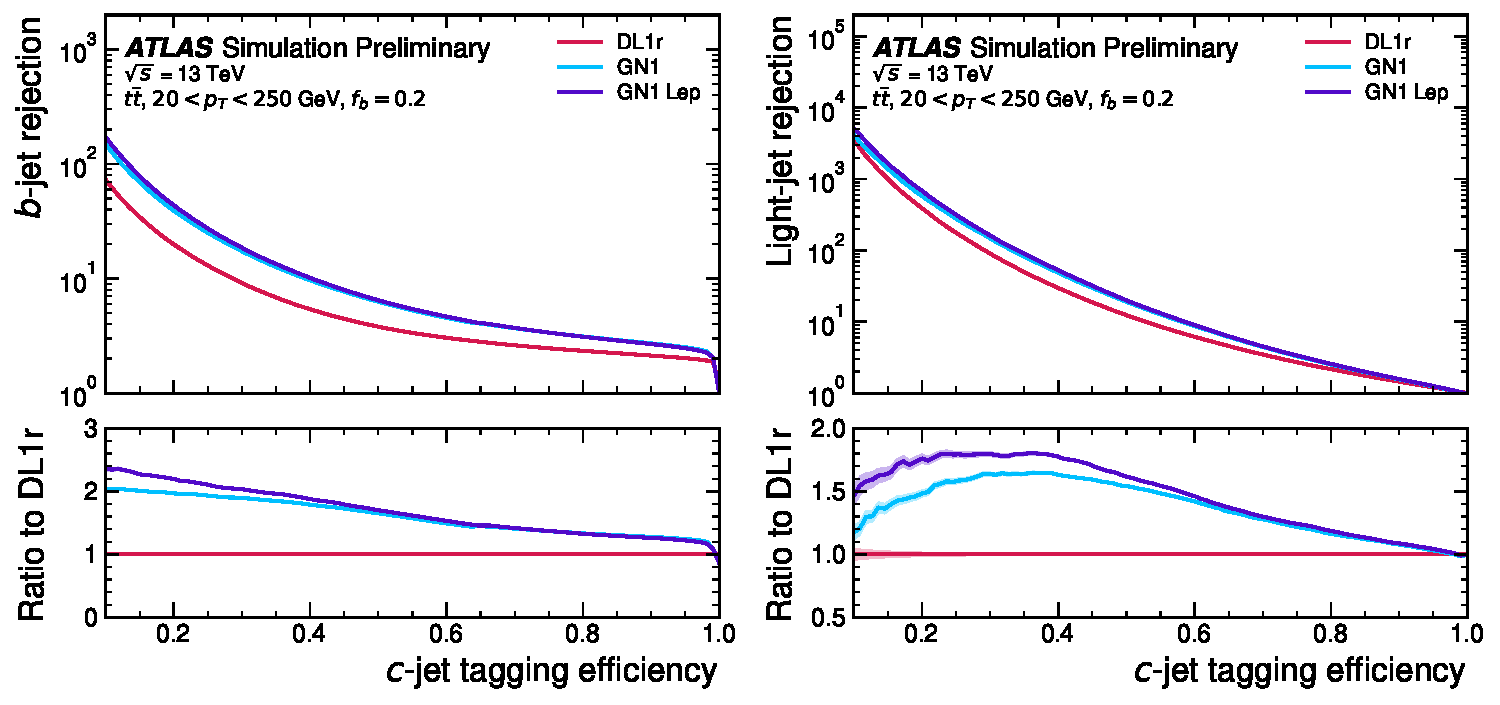
\includegraphics[width=\textwidth]{chapters/gnn_tagger/figs/results/main/ttbar/ttbar_roc_ctag.pdf}
    \caption{The \bjet (left) and \ljet (right) rejections as a function of the $c$-jet tagging efficiency for \ttbar jets with \ttbarpt.
             The ratio to the performance of the \DLr algorithm is shown in the bottom panels.
             Binomial error bands are denoted by the shaded regions.
             At $c$-jet tagging efficiencies than $\sim$\pct{25}, the \lrej becomes so large that the effect of the low number of jets is visible.
             The lower $x$-axis range is chosen to display the \cjet tagging efficiencies usually probed in these regions of phase space.}
    \label{fig:ttbar_ctag_roc}
\end{figure}

\begin{figure}[!p]
   \centering
   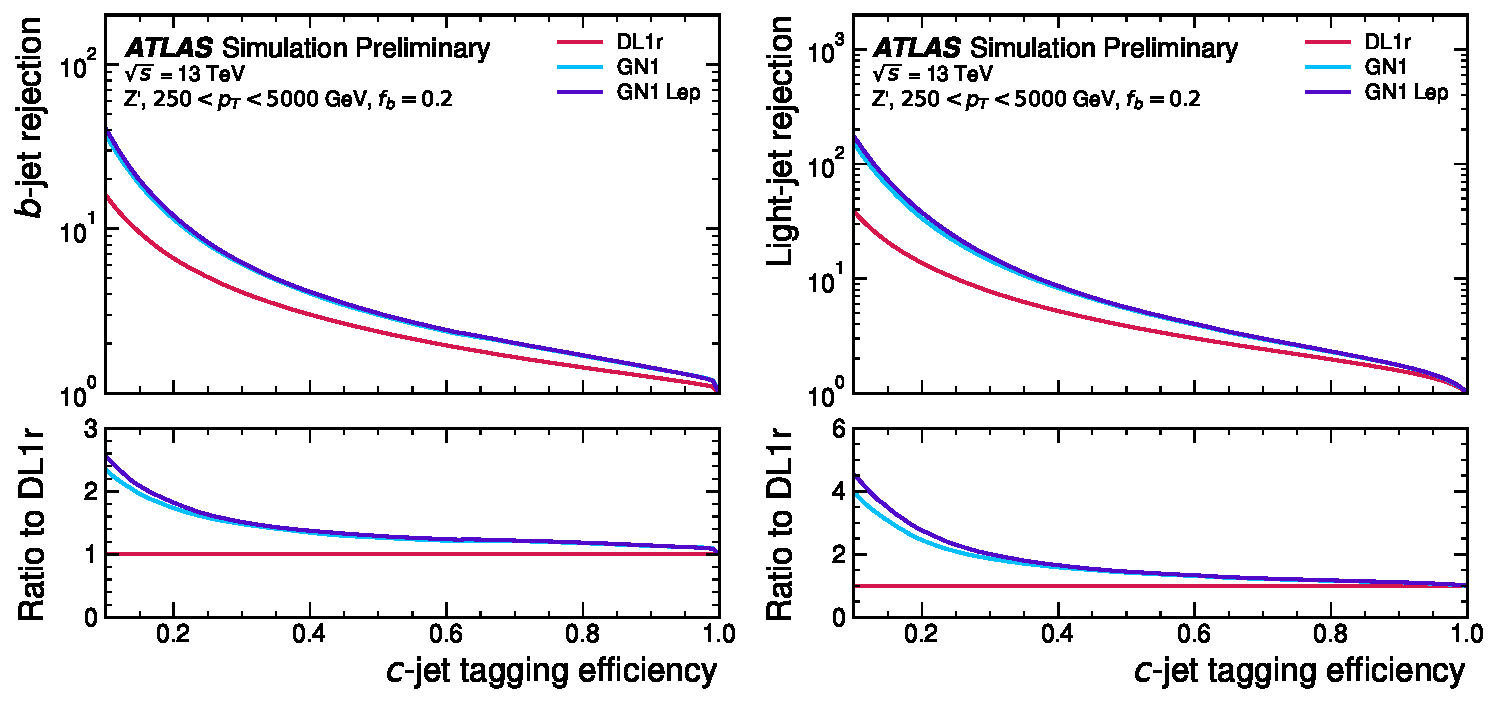
\includegraphics[width=\textwidth]{chapters/gnn_tagger/figs/results/main/zprime/zprime_roc_ctag.pdf}
   \caption{The \bjet (left) and \ljet (right) rejections as a function of the $c$-jet tagging efficiency for \Zprime jets with \Zprimept.
            The ratio to the performance of the \DLr algorithm is shown in the bottom panels.
            Binomial error bands are denoted by the shaded regions.
            The lower $x$-axis range is chosen to display the \cjet tagging efficiencies usually probed in these regions of phase space.}
   \label{fig:zprime_ctag_roc}
\end{figure}




\subsection{Ablations}\label{sec:gnn_ablations}

Several ablations, the removal of components in the model to study their impact, are carried out to determine the importance of the auxiliary training objectives of \GNN to the overall performance.
The ``\GNN No Aux'' variant retains the primary jet classification objective, but removes both track classification and vertexing auxiliary objectives (see \cref{sec:aux-train-objectives}) and as such only minimises the jet classification loss.
The ``\GNN TC'' variant includes track classification but not vertexing, while ``\GNN Vert'' includes vertexing, but not track classification.

For jets in both the \ttbar and \Zprime samples, the models without one or both of the auxiliary objectives display significantly reduced \clrej when compared with the baseline \GNN model, as shown in \cref{fig:ttbar_btag_roc_ab,fig:zprime_btag_roc_ab}.
For \ttbarjets, the performance of \GNN No Aux is similar to \DLr, while \GNN TC and \GNN Vert perform similarly to each other.
% with improvements in the \crej of \pct{80} and improvements in the \lrej of \pct{75} at a $b$-jet tagging efficiency of \pct{60}.
For \Zprimejets, the \GNN No Aux model shows a clear improvement in \clrej when compared with \DLr at lower $b$-jet tagging efficiencies.
Similar to \ttbarjets, \GNN TC and \GNN Vert perform similarly, and bring large gains in background rejection when compared with \GNN No Aux, but the combination of both auxiliary objectives yields the best performance.

It is notable that the \GNN No Aux model matches or exceeds the performance of \DLr without the need for inputs from the low-level algorithms.
This indicates that the performance improvements enabled by \GNN appear to be able to compensate for the removal of the low-level algorithm inputs.
The \GNN TC and \GNN Vert variants each similarly outperform \DLr, demonstrating that both contribute to the overall high performance of the baseline model.


\begin{figure}[!p]
    \centering
    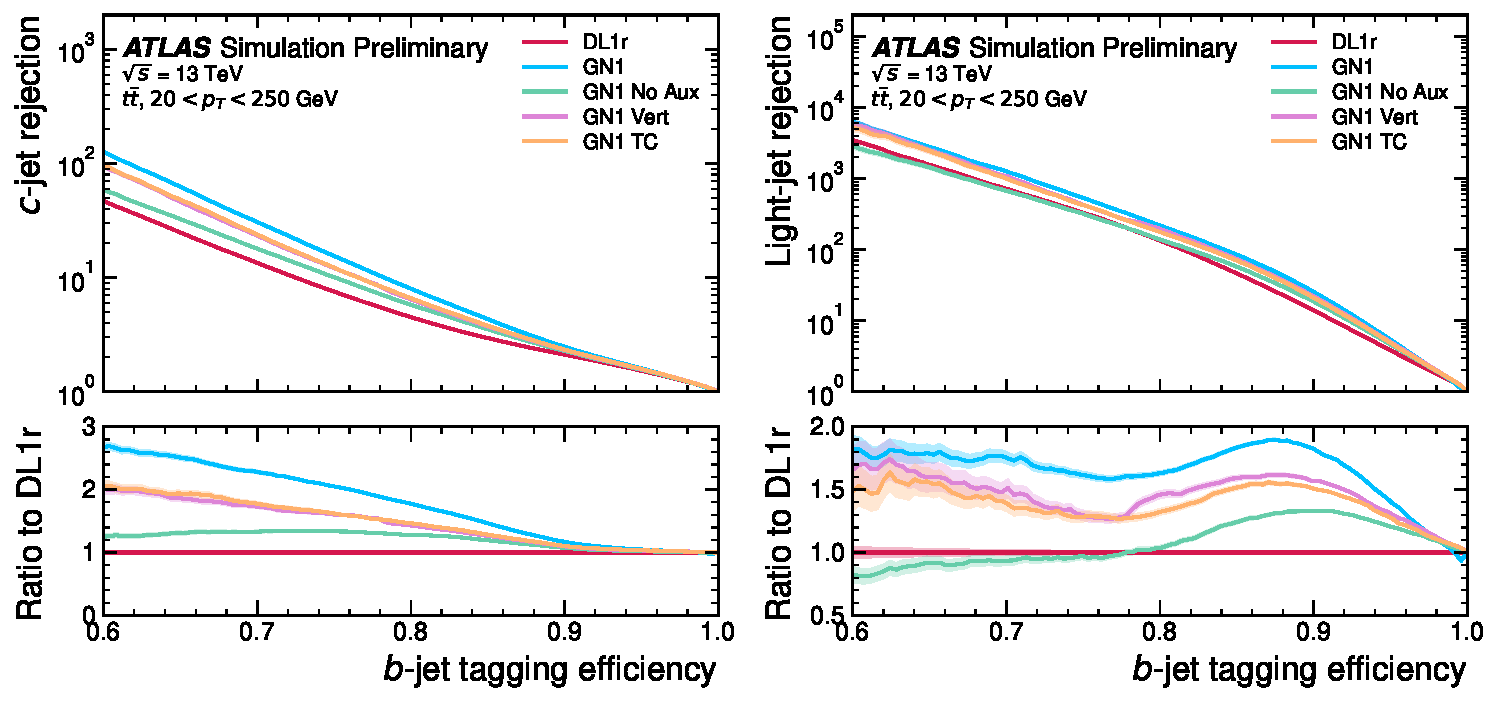
\includegraphics[width=\textwidth]{chapters/gnn_tagger/figs/results/ablations/ttbar/ttbar_roc_btag.pdf}
    \caption{The \cjet (left) and \ljet (right) rejections as a function of the \bjet tagging efficiency for \ttbar jets with \ttbarpt, for the nominal \GNN, in addition to configurations where no (\GNN No Aux), only the track classification (\GNN TC) or only the vertexing (\GNN Vert) auxiliary objectives are deployed. The ratio to the performance of the \DLr algorithm is shown in the bottom panels. A value of $\fc = 0.018$ is used in the calculation of \Db for \DLr and $\fc = 0.05$ is used for \GNN. Binomial error bands are denoted by the shaded regions. At \bjet tagging efficiencies less than $\sim65\%$, the \lrej become so large that the effect of the low number of jets are visible. The lower $x$-axis range is chosen to display the \bjet tagging efficiencies usually probed in these regions.}
    \label{fig:ttbar_btag_roc_ab}
\end{figure}

\begin{figure}[!p]
    \centering
    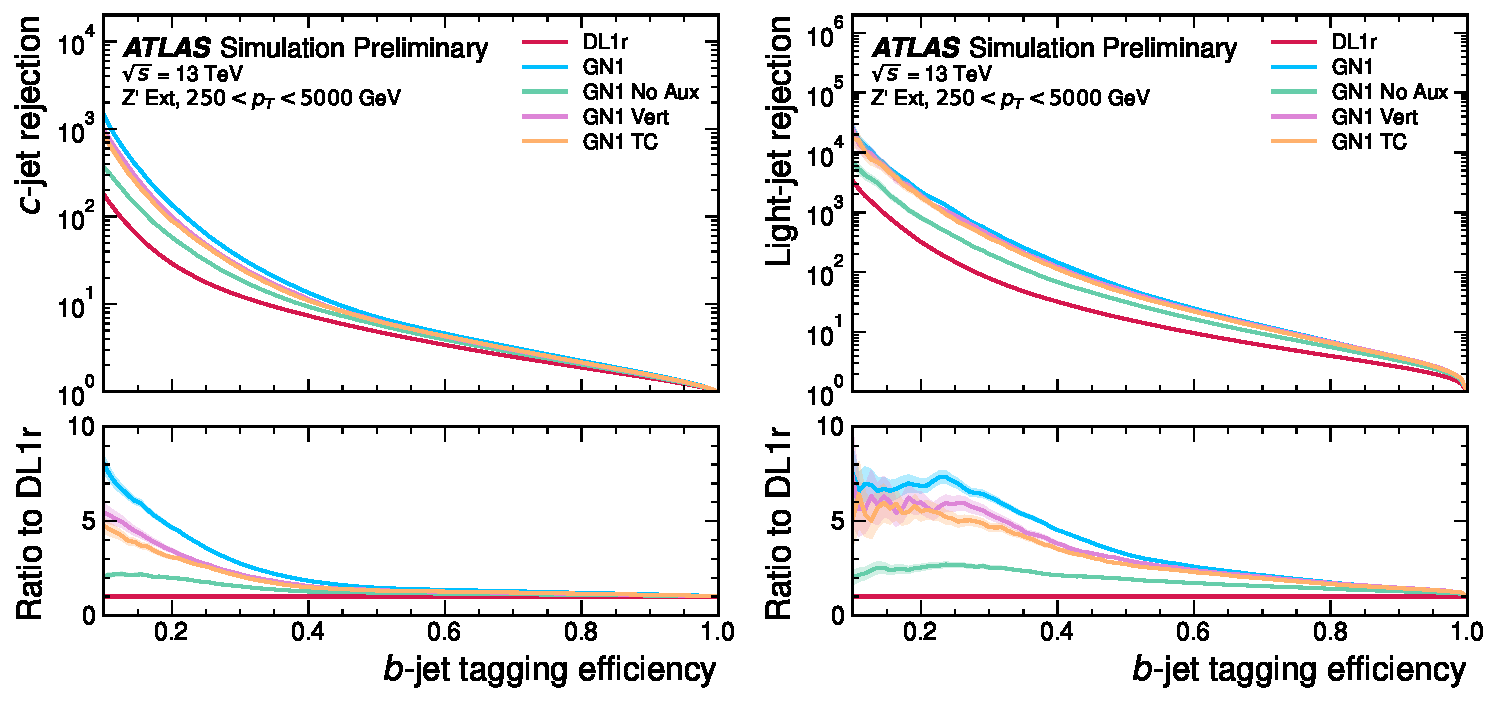
\includegraphics[width=\textwidth]{chapters/gnn_tagger/figs/results/ablations/zprime/zprime_roc_btag.pdf}
    \caption{The \cjet (left) and \ljet (right) rejections as a function of the \bjet tagging efficiency for \Zprime jets with \Zprimept, for the nominal \GNN, in addition to configurations where no (\GNN No Aux), only the track classification (\GNN TC) or only the vertexing (\GNN Vert) auxiliary objectives are deployed. The ratio to the performance of the \DLr algorithm is shown in the bottom panels. A value of $\fc = 0.018$ is used in the calculation of \Db for \DLr and $\fc = 0.05$ is used for \GNN. Binomial error bands are denoted by the shaded regions. At \bjet tagging efficiencies less than $\sim25\%$, the \lrej become so large that the effect of the low number of jets are visible. The lower $x$-axis range is chosen to display the \bjet tagging efficiencies usually probed in these regions.}
    \label{fig:zprime_btag_roc_ab}
\end{figure}



\subsection{Inclusion of Low-Level Vertexing Algorithms}\label{sec:gnn_low_level_vert_impact}

\GNN does not include inputs from low-level tagging algorithms, including the vertexing tools SV1 and JetFitter \cite{FTAG-2018-01}.
Since these algorithms are known to improve the performance of \DLr, it was feasible that their inclusion in \GNN may further improve on the performance of the \GNN models.
In a dedicated training of \GNN the SV1 and JetFitter tagger outputs were added to the \GNN jet classification network as an input, similar to their use in \DLr.
These outputs include information on the reconstructed vertices, including the number of vertices, the vertex mass, displacement, and other properties.
In addition, the index of the reconstructed SV1 or JetFitter vertices were included as two track-level inputs to \GNN. 
%These indices were also used to construct an edge feature for the edge classification network, which was given a value of one if the track-pair were from a common reconstructed V1 or JetFitter vertex, and zero otherwise.
The jet classification performance of this \GNN model was not significantly different to the baseline model, and in some cases the performance was slightly reduced.
%As \GNN does not benefit from the inclusion of information from SV1 and JetFitter it can function as a highly performant standalone tagger that does not require (beyond etraining) any manual optimisation to achieve good performance in a wide range of phase spaces.
A dedicated look at the vertexing performance of \GNN with some comparisons to SV1 and JetFitter is found in \cref{sec:gnn_vert_perf}







\subsection{Vertexing Performance}\label{sec:gnn_vert_perf}

From the track-pair vertex prediction described in \cref{sec:aux-train-objectives}, tracks can be partitioned into compatible groups representing vertices (see \cite{serviansky2020set2graph}).
As such, \GNN is able to be used to perform vertex ``finding'', but not vertex ``fitting'', i.e. the reconstruction of a vertex's properties, which currently still requires the use of a dedicated vertex fitter.
In order to study the performance of the different vertexing tools inside \bjets, the truth vertex label of the tracks, discussed in \cref{sec:aux-train-objectives}, are used.
To estimate the efficiency with which \GNN manages to find vertices inclusively, vertices from \GNN containing tracks identified as coming from a \bhadron are merged together and compared to the inclusive truth decay vertices that result from a \bhadron decay (where if there are multiple distinct truth vertices from a \bhadron decay they are also merged together).
Vertices are compared with the target truth vertex and the number of correctly and incorrectly assigned tracks is computed.
Since secondary vertex information is only recovered for reconstructed tracks, an efficiency of $100\%$ here denotes that all possible secondary vertices are recovered given the limited track reconstruction efficiency.
A vertex is considered matched if it contains at least $65\%$ of the tracks in the corresponding truth vertex, and has a purity of at least $50\%$.
\GNN manages to achieve an inclusive reconstruction efficiency in \bjets of $\sim80\%$, demonstrating that it effectively manages to identify the displaced vertices from \bhadron decays.

\subsubsection{More detail}

In order to study the performance of the different vertexing tools inside \bjets, the truth vertex label of the tracks, discussed in \cref{sec:aux-train-objectives}, is used.
The reconstructed vertices from \GNN, SV1 and JetFitter are compared to the target truth vertices in order to calculate the efficiencies of the different vertexing tools.
Since secondary vertex information is only recovered for reconstructed tracks, an efficiency of $100\%$ here denotes that all possible secondary vertices are recovered given the limited track reconstruction efficiency.

There are several caveats to a comparison of the vertexing tools which are a result of the different approaches they take to vertexing.
SV1 and JetFitter are designed to only find secondary vertices in the jet, whereas \GNN is also trained to determine which tracks in the jet belong to the primary vertex (the vertex of the hard scatter $pp$ interaction).
To account for this the \GNN vertex with the largest number of predicted primary tracks is excluded from the vertex finding efficiency calculation.
While JetFitter and \GNN aim to resolve each displaced vertex inside the jet, such that secondary vertices from \bhadron decays are found separately to tertiary vertices from $b \rightarrow c$ decay chains, SV1 by design attempts to find a single inclusive vertex per jet.
This inclusive vertex groups inclusive \bhadron decays.
These are tracks from the \bhadron decay itself (FromB) and tracks from $b \rightarrow c$ decays (FromBC).
In order to fairly compare the performance if the different tools, both the exclusive and inclusive vertex finding efficiency is studied.
For the exclusive vertex finding case JetFitter and \GNN can be directly compared, while a comparison with SV1 is not possible due to aforementioned design constraints.
The inclusive vertex finding performance of all three tools can be compared using the procedure outlined below.

The starting point for the secondary vertex finding efficiency in both the exclusive and inclusive cases is to select truth secondary vertices are those containing only inclusive \bhadron decays to be considered as initial targets.
For exclusive vertex finding, these truth secondary vertices can be used directly as the demoninator for the efficiency calculation.
Meanwhile for the inclusive efficiency all such truth secondary vertices in the jet are merged into a single inclusive target vertex.
Correspondingly, for the inclusive vertex finding case, the vertices found by JetFitter are merged into a single vertex, and the vertices found by \GNN with at least one predicted inclusive \bhadron decay track are also merged similarly.
SV1 does not require any vertex merging.

Next, in both cases for each truth secondary vertex, vertices in the jet found by the different vertexing tools are compared with the target truth vertex.
The number of correctly and incorrectly assigned tracks is computed.
In order to call a vertex efficient, it is required to contain at least $65\%$ of the tracks in the corresponding truth vertex, and to have a purity of at least $50\%$.
Single track vertices are required to have a purity of $100\%$.
Additionally, for \GNN only, at least one track in the vertex is required to have a predicted heavy flavour origin.


\begin{figure}[!htbp]
    \centering
    \begin{subfigure}[b]{0.48\textwidth}
        \centering
        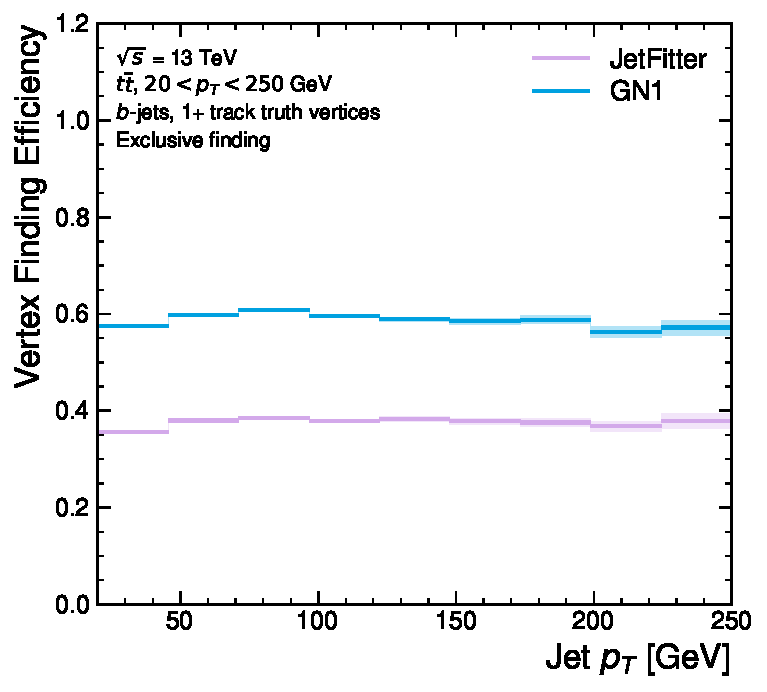
\includegraphics[width=\textwidth]{chapters/gnn_tagger/figs/results/tracks/ttbar/ttbar_bjet_vert_eff_1+_track_excl.pdf}
        %\caption{sub}
        %\label{fig:sub}
    \end{subfigure}
    \quad
    \begin{subfigure}[b]{0.48\textwidth}
        \centering
        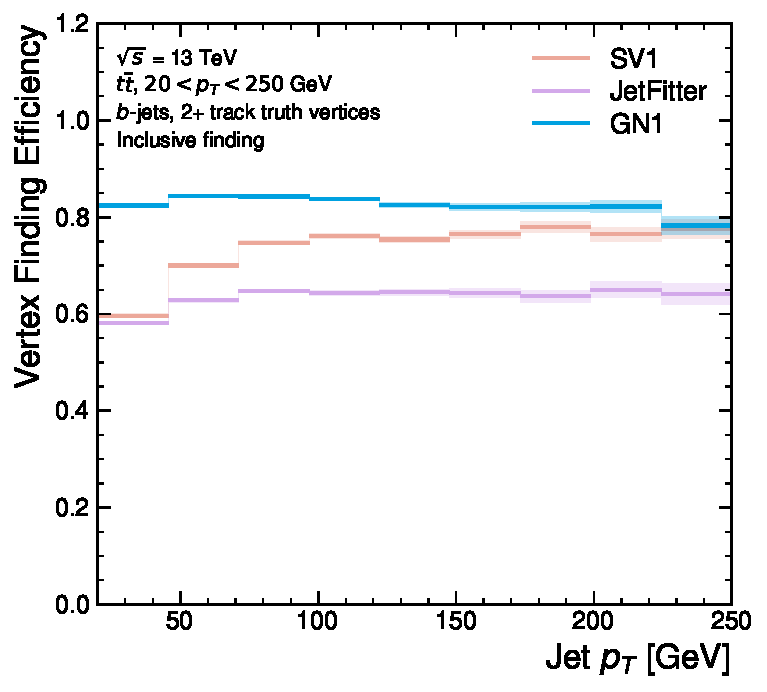
\includegraphics[width=\textwidth]{chapters/gnn_tagger/figs/results/tracks/ttbar/ttbar_bjet_vert_eff_2+_track_incl.pdf}
        %\caption{sub}
        %\label{fig:sub}
    \end{subfigure}
    \caption{Vertex finding efficiency as a function of jet \pt for \ttbarbjets using the exclusive (left) and inclusive (right) vertex finding approaches.
             Efficient vertex finding requires the recall of at least $65\%$ of the tracks in the truth vertex, and allows no more than $50\%$ of the tacks to be included incorrectly.
             Binomial error bands are denoted by the shaded regions.}
    \label{fig:ttbar_vert_eff}
\end{figure}

Vertex finding efficiencies for \ttbarbjets are displayed as a function of \pt separately for the inclusive and exclusive approaches in \cref{fig:ttbar_vert_eff}.
For \ttbarbjets with \ttbarpt, the exclusive vertex finding efficiency of JetFitter and \GNN is relatively flat as a function of \pt.
Of the truth secondary vertices in this \pt region, JetFitter efficiently finds approximately \pct{40} and \GNN finds approimately \pct{55}.
When finding vertices inclusively the vertex finding efficiency is generally higher.
An increased dependence on \pt is also visible for JetFitter and SV1. As the jet \pt increases from \SI{20}{\GeV} to \SI{100}{\GeV}, the efficiency of JetFitter increases from \pct{55} to \pct{65}.
In the same range, the efficiency of SV1 increases from \pct{55} to \pct{75}.
\GNN displays less dependence on \pt than JetFitter and SV1, efficiently finding upwards of \pct{80} of vertices in \bjets in this \pt region. 
For \bjets with $\pt > \SI{100}{\GeV}$, JetFitter finds approximately \pct{65} of vertices, SV1 finds approimately \pct{75} of vertices, and \GNN finds approximately \pct{80} of vertices.

For \Zprimebjets, the vertex finding efficiency drops steeply with increasing \pt up until $\pt = \SI{3}{\TeV}$.
\GNN outperforms SV1 and JetFitter across the \pt spectrum.
In the first bin, the efficiency of \GNN is $75\%$, while the efficiencies of SV1 and JetFitter are around $60\%$.
The efficiency of SV1 drops rapidly to almost zero above \SI{3}{\TeV}, while JetFitter and \GNN retain approximately $30\%$ efficiency.
\cref{fig:zprime_vert_eff} compares the exclusive vertex finding efficiencies of JetFitter and \GNN for multitrack vertices.
JetFitter finds $45\text{\nobreakdash-}50\%$ of vertices in \ttbarbjets, while \GNN finds $60\text{\nobreakdash-}65\%$.
For \Zprimebjets, JetFitter finds $35\%$ of vertices in the first bin, dropping to $20\%$ of vertices above \SI{2}{\TeV}.
\GNN finds $55\%$ of vertices in the first bin, dropping to $30\%$ above \SI{2}{\TeV}.


\begin{figure}[!htbp]
    \centering
    \begin{subfigure}[b]{0.48\textwidth}
        \centering
        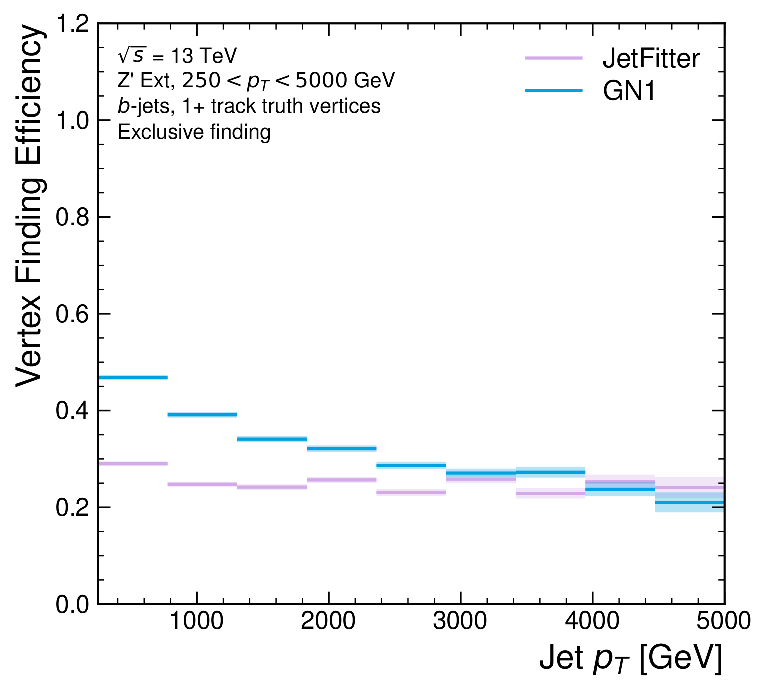
\includegraphics[width=\textwidth]{chapters/gnn_tagger/figs/results/tracks/zprime/zprime_bjet_vert_eff_1+_track_excl.pdf}
        %\caption{sub}
        %\label{fig:sub}
    \end{subfigure}
    \quad
    \begin{subfigure}[b]{0.48\textwidth}
        \centering
        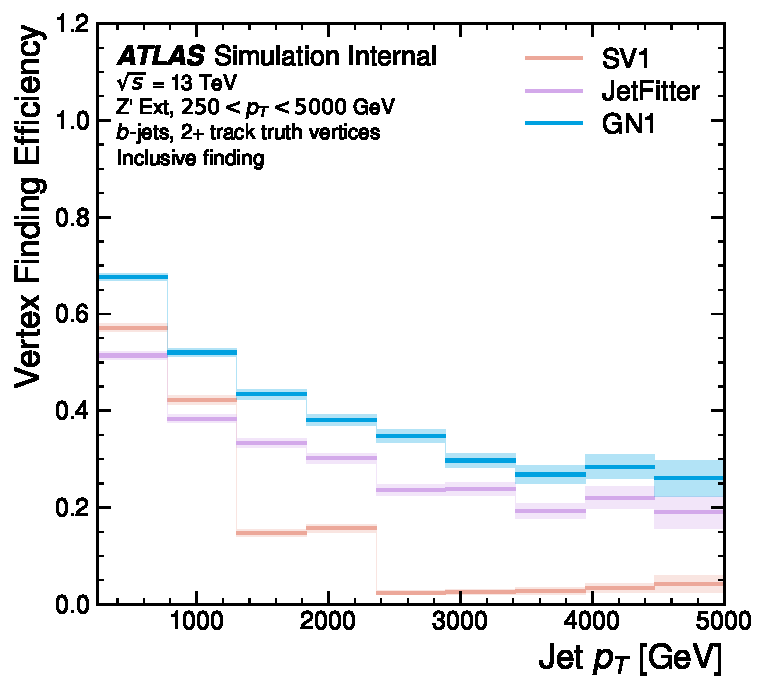
\includegraphics[width=\textwidth]{chapters/gnn_tagger/figs/results/tracks/zprime/zprime_bjet_vert_eff_2+_track_incl.pdf}
        %\caption{sub}
        %\label{fig:sub}
    \end{subfigure}
    \caption{Inclusive vertex finding efficiency for multitrack truth vertices in \ttbarbjets (left) and \Zprimejets (right) as a function of jet \pt. Efficient vertex finding requires the recall of at least $65\%$ of the tracks in the truth vertex, and allows no more than $50\%$ of the tacks to be included incorrectly.}
    \label{fig:zprime_vert_eff}
\end{figure}


%\GNN also outperforms JetFitter in single track exclusive vertex finding as shown in \cref{fig:vert_eff_1track_excl}, except at $\pt > 3 ~\TeV$, where the efficiency of JetFitter starts to increase.
%As shown in \cref{fig:vert_eff_1track_excl}, JetFitter has a high rate to find vertices in \ljets in this region of phase space.
%\cref{fig:vert_eff_1track_excl} shows the rate at which the different tools find vertices within \ljets as a function of jet \pt. 
%Found vertices in \ljets can correspond to real displaced truth vertices caused by for example material interactions, or can be comprised of tracks which do not originate from a common displaced truth vertex (``fake'' vertices).
%The SV1 rate remains low at under $10\%$ for \ttbarZprimeljets.
%
%\begin{figure}[!htbp]
%    \centering
%    \begin{subfigure}[b]{0.48\textwidth}
%        \centering
%        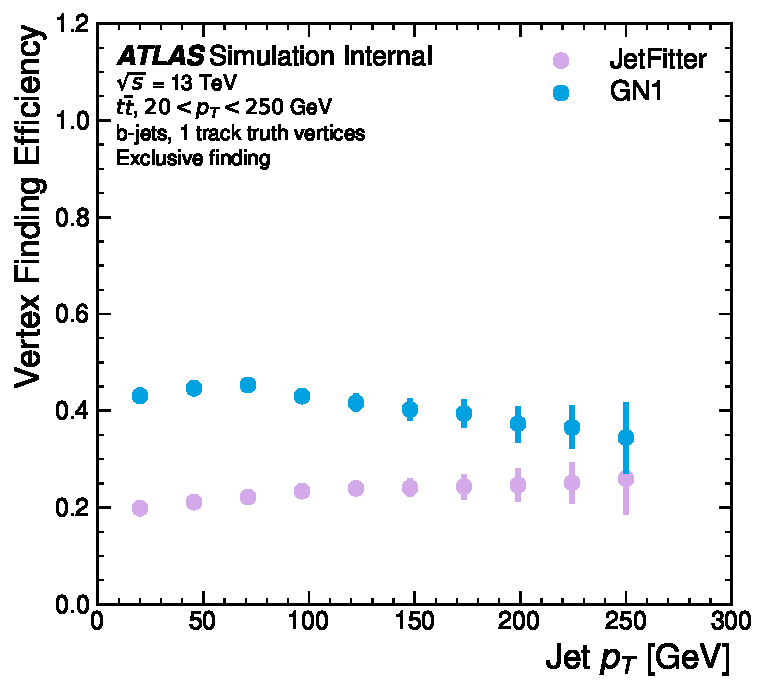
\includegraphics[width=\textwidth]{fig/results/tracks/ttbar/ttbar_vert_eff_1_track_excl.pdf}
%        %\caption{sub}
%        %\label{fig:sub}
%    \end{subfigure}
%    \quad
%    \begin{subfigure}[b]{0.48\textwidth}
%        \centering
%        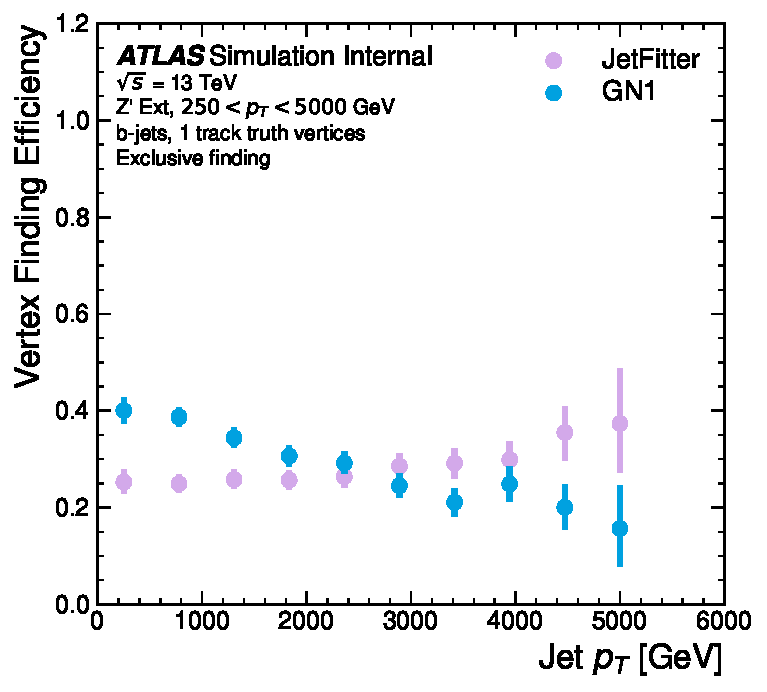
\includegraphics[width=\textwidth]{fig/results/tracks/zprime/zprime_vert_eff_1_track_excl.pdf}
%        %\caption{sub}
%        %\label{fig:sub}
%    \end{subfigure}
%    \caption{Exclusive vertex finding efficiency for single track truth vertices in \ttbarbjets (left) and \Zprimejets (right) as a function of jet \pt. Efficient vertex finding in single track vertices requires the truth and found vertex to match exactly.}
%    \label{fig:vert_eff_1track_excl}
%\end{figure}
%
%For \ttbarljets, the rate of found JetFitter (\GNN) vertices increases as a function of \pt from 0.3 to 0.7 (0.5 to 1.1) vertices per jet.
%For \Zprimeljets, the vertexing rate of JetFitter plateaus above $3 ~\TeV$ at 2 vertices per jet, while the \GNN rate decreases steadily from 1.4 vertices for $\pt < 1 ~\TeV$ to 0.8 vertices above $4 ~\TeV$.
%By requiring that vertices found by \GNN also include at least one track with a predicted heavy flavour origin, as was done for the vertexing efficiency, the rate of \GNN vertices in \ljets can be suppressed to levels similar as found by SV1.
%Overall these results indicate that the \GNN model is able to efficiency find vertices when compared with SV1 and JetFitter.
%
%\begin{figure}[!htbp]
%    \centering
%    \begin{subfigure}[b]{0.48\textwidth}
%        \centering
%        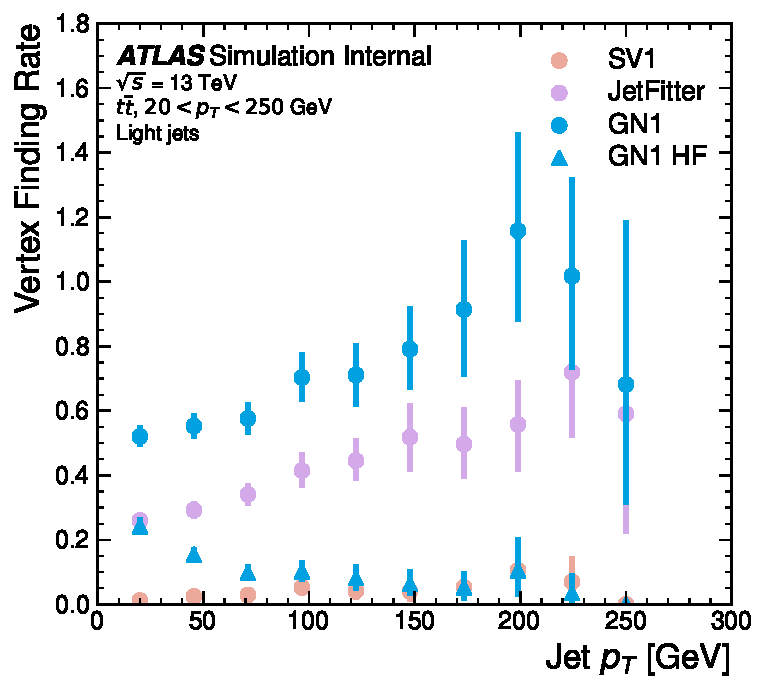
\includegraphics[width=\textwidth]{fig/results/tracks/ttbar/ttbar_vert_fake_all_v2.pdf}
%        %\caption{sub}
%        %\label{fig:sub}
%    \end{subfigure}
%    \quad
%    \begin{subfigure}[b]{0.48\textwidth}
%        \centering
%        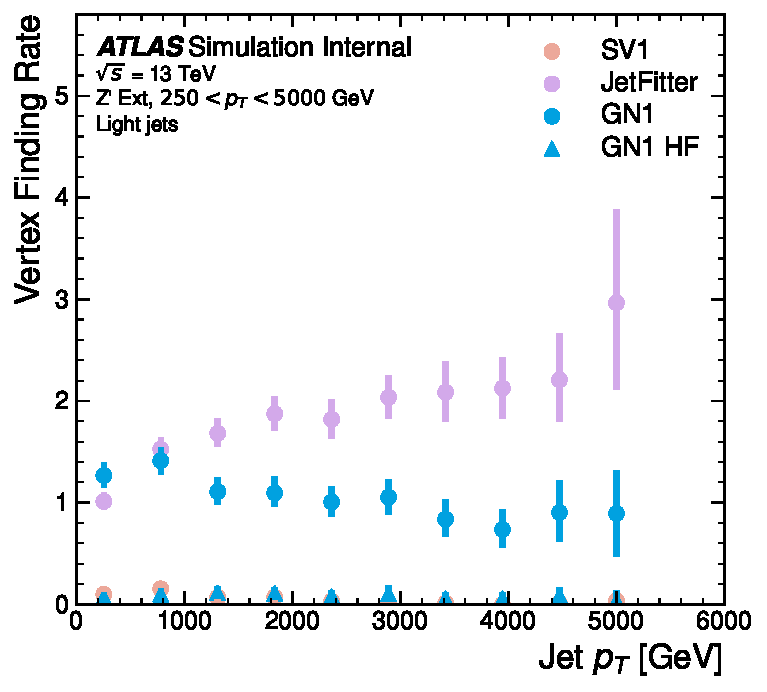
\includegraphics[width=\textwidth]{fig/results/tracks/zprime/zprime_vert_fake_all_v2.pdf}
%        %\caption{sub}
%        %\label{fig:sub}
%    \end{subfigure}
%    \caption{Vertex finding rate in \ljets for truth vertices in \ttbarbjets (left) and \Zprimejets (right) as a function of jet \pt. Found vertices in \ljets can correspond to real displaced vertices from secondary interactions or can be fake vertices. \GNN has a relatively high rate to find vertices in \ljets, though this can be suppressed by requiring that at least one track in the vertex have a predicted heavy flavour origin.}
%    \label{fig:vert_fake_all}
%\end{figure}



\subsection{Track Classification Performance}\label{sec:gnn_tc_perf}

As discussed in \cref{sec:aux-train-objectives}, one of the auxiliary training objectives for \GNN is to predict the truth origin of each track in the jet.
Since the equivalent information is not provided by any of the existing flavour tagging tools, as a benchmark a multi-class classification multilayer perceptron (MLP) is trained on the same tracks used for the baseline \GNN training.
The model uses the same concatenated track-and-jet inputs as \GNN (see \cref{sec:model-inputs}), but processes only a single track at a time.
The model is comprised of five densely connected layers with 200 neurons per layer, though the performance was not found to be strongly sensitive to changes in the network structure. 
To measure the track classification performance, the area under the curve (AUC) of the receiver operating characteristic (ROC) curve is computed for each origin class using a one versus all classification approach.
The AUCs for the different truth origin classes are averaged using both an unweighted and a weighted approach.
%Several metrics are used to measure the performance of the two models in \cref{tab:track_classification_metrics}, where the performance for the different truth origin classes is averaged over using both an unweighted and a weighted approach.
The unweighted mean treats the performance of each class equally, while the weighted mean uses the fraction of tracks from each origin as a weight.
As seen in \cref{tab:track_classification_metrics}, \GNN outperforms the MLP, both at \ttbarpt for \ttbarjets, and at \Zprimept for \Zprimejets.
For tracks in \ttbarjets, \GNN can reject \pct{65} of fake tracks while retaining more than \pct{99} of good tracks.
The \GNN model has two advantages over the MLP which can explain the performance improvement.
Firstly, the mixing of information between tracks, enabled by the fully connected graph network architecture as discussed in \cref{sec:Architecture}, is likely to be beneficial since the origins of different tracks within a jet are to some extent correlated.
Secondly, the jet classification and vertexing objectives can be considered auxiliary to the track classification task, and may bring improved track classification performance with respect to the standalone MLP.

\begin{table}[!htbp]
  \footnotesize\centering
  \setlength{\tabcolsep}{0.5em} % for the horizontal padding
  \caption{The area under the ROC curves (AUC) for the track classification from \GNN, compared to a standard multilayer perceptron (MLP) trained on a per-track basis. 
            The unweighted mean AUC over the origin classes and weighted mean AUC (using as a weight the fraction of tracks from the given origin) is provided.
            \GNN, which uses an architecture that allows track origins to be classified in a conditional manner as discussed in \cref{sec:Architecture}, outperforms the MLP model for both \ttbar and \Zprime jets.}
  \begin{tabular}{cccccccccc}
      \toprule 
      \multicolumn{1}{l}{}    & \multicolumn{1}{l}{} & \multicolumn{2}{c}{AUC}\\%                               & \multicolumn{2}{c}{Precision}                           & \multicolumn{2}{c}{Recall}                              & \multicolumn{2}{c}{F1}                                  \\
      \multicolumn{1}{l}{}    & \multicolumn{1}{l}{} & \multicolumn{1}{c}{Mean} & \multicolumn{1}{c}{Weighted}\\% & \multicolumn{1}{c}{Mean} & \multicolumn{1}{c}{Weighted} & \multicolumn{1}{c}{Mean} & \multicolumn{1}{c}{Weighted} & \multicolumn{1}{c}{Mean} & \multicolumn{1}{c}{Weighted} \\
      \cmidrule(lr){3-4}% \cmidrule(lr){5-6} \cmidrule(lr){7-8} \cmidrule(lr){9-10}

      \multirow{2}{*}{\ttbar} & 
      MLP & 0.87 & 0.89 \\ & %& 0.39 & 0.71 & 0.51 & 0.56 & 0.36 & 0.62 \\ & 
      GN1 & \textbf{0.92} & \textbf{0.95} \\% & \textbf{0.51} & \textbf{0.82} & \textbf{0.64} & \textbf{0.70} & \textbf{0.51} & \textbf{0.74} 
      \\
      \multirow{2}{*}{\Zprime} & 
      MLP & 0.90 & 0.94 \\ & %& 0.36 & 0.84 & 0.47 & 0.72 & 0.31 & 0.76 \\ &
      GN1 & \textbf{0.94} & \textbf{0.96} \\% & \textbf{0.48} & \textbf{0.88} & \textbf{0.60} & \textbf{0.79} & \textbf{0.48} & \textbf{0.82} \\             
      \bottomrule
  \end{tabular}
  \vspace{4mm}
  \label{tab:track_classification_metrics}
\end{table}


\cref{fig:track_origin_roc} shows the track origin classification ROC curves for the different track origins for \ttbarZprimejets.
In order to improve legibility of the figure, the heavy flavour truth origins have been combined weighted by their relative abundance, as have the Primary and OtherSecondary labels.
In \ttbarZprimejets, the AUC of the different (grouped) origins is above $0.9$, representing good classification performance.
Fake tracks, followed by pileup tracks, are the easiest to classify in both samples.
%the FromC tracks which are \chadron decay products, are the hardest to classify, possibly due to their similarity to both fragmentation tracks and \bhadron decay tracks, depending on the \chadron in question.

\begin{figure}[!htbp]
    \centering
    \begin{subfigure}[b]{0.48\textwidth}
        \centering
        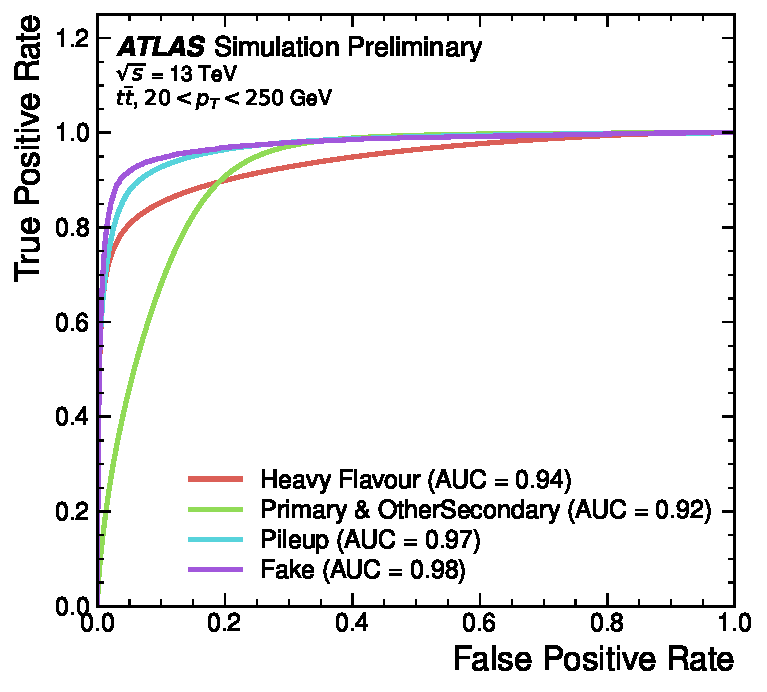
\includegraphics[width=\textwidth]{chapters/gnn_tagger/figs/results/tracks/ttbar/ttbar_origin_roc_GNNv11.pdf}
        %\caption{sub}
        %\label{fig:sub}
    \end{subfigure}
    \quad
    \begin{subfigure}[b]{0.48\textwidth}
        \centering
        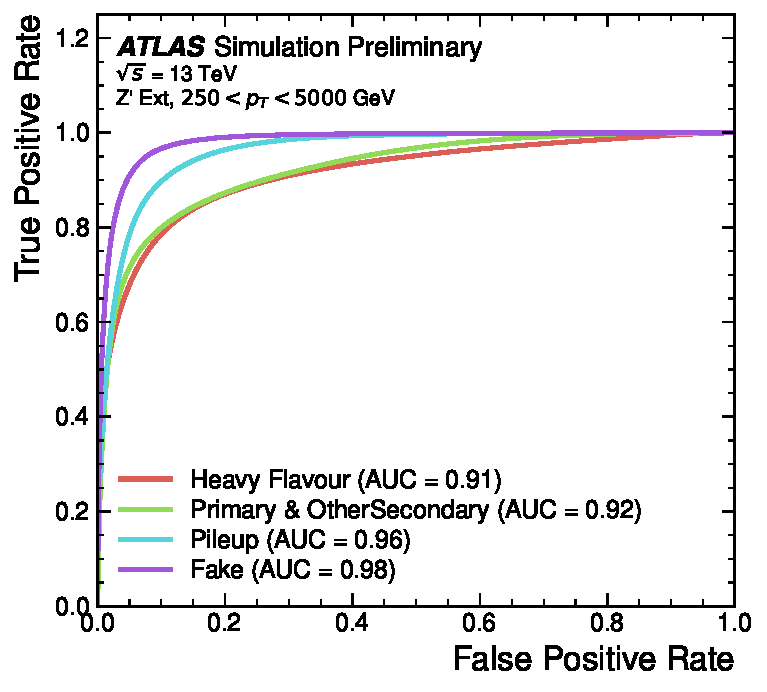
\includegraphics[width=\textwidth]{chapters/gnn_tagger/figs/results/tracks/zprime/zprime_origin_roc_GNNv11.pdf}
        %\caption{sub}
        %\label{fig:sub}
    \end{subfigure}
    \caption{ROC curves for the different groups of truth origin labels defined in \cref{tab:truth_origins} for \ttbarjets (left) and \Zprimejets (right).
             The FromB, FromBC and FromC labels have been combined, weighted by their relative abundance, into the Heavy Flavour category, and the Primary and OtherSecondary labels have similarly been combined into a single category.
             The mean weighted area under the ROC curves (AUC) is similar for both samples.}
    \label{fig:track_origin_roc}
\end{figure}


\section{Conclusion}\label{sec:gnn_conclusion}


A novel jet tagger, \GNN, with a graph neural network architecture and trained with auxiliary training targets, is presented and now fully implemented in the ATLAS software.
\GNN is shown to improve flavour tagging performance with respect to \DLr, the current default ATLAS flavour tagging algorithm, when compared in simulated collisions.
\GNN improves \clrej for \ttbarjets with \ttbarpt by factors of \ttbclo and \ttbllo respectively at a \bjet tagging efficiency of $70\%$ when compared with \DLr.
For \Zprimejets with \Zprimept, \GNN improves the \crej by a factor of \zpbclo and \lrej by a factor of \zpbllo for a comparative \bjet efficiency of $30\%$.
Previous multivariate flavour tagging algorithms relied on inputs from low-level tagging algorithms, whereas \GNN needs no such inputs, making it more flexible. It can be easily fully optimised via a retraining for specific flavour tagging use cases, as demonstrated with \ctag and high-\pt \btag, without the need for time-consuming retuning of the low-level tagging algorithms.
The model is also simpler to maintain and study due to the reduction of constituent components.
\GNN demonstrates improved track classification performance when compared with a simple per-track MLP and an efficiency of $\sim80\%$ for inclusive vertex finding in \bjets.
The auxiliary track classification and vertex finding objectives are shown to significantly contribute to the performance in the jet classification objective, and are directly responsible for the improvement over \DLr.
Further studies need to be undertaken to verify the performance of \GNN on collision data.
%Due to good performance and relative ease of optimisation, application of a GNN model could lead to improved performance for other use cases extending beyond standard $b$- and \ctag applications.
%The flexible nature of the \GNN model may make it a good candidate for other tasks, such as $X \rightarrow bb$ and $X \rightarrow cc$ tagging, and vertexing for long lived particle decays. Exporing the application of \GNN to these tasks is left for future work.


\section{Extensions}
\subsection{Looser Track Selection}